\chapter{Обзор литературы} \label{chapt1}

\section{Архитектура генома прокариот} \label{sect1_1}
Понятие геном было введено немецким ботаником Гансом Винклером в 1920-м году для обозначения гаплоидного набора хромосом в ядре эукариотической клетки \cite{noguera2013genome}. Считается, что слово было образовано за счет объединения терминов "ген"\ и ``хромосома''. Сейчас, у прокариот под геномом понимают генетическую информацию, которая находится в фрагментах ДНК, способных к репликации --- репликонах --- хромосоме (одной или нескольких), и в плазмидах (при их наличии).  

Как правило, геном прокариот представлен одной кольцевой хромосомой; также в клетке может находиться одна либо несколько плазмид. Есть и исключения из этого правила. Существуют бактериальные виды с несколькими хромосомами, например, у холерного вибриона (\textit{Vibrio cholerae}) есть две хромосомы \cite{trucksis1998vibrio}. Необычно организован геном бактерии \textit{Borrelia burgdorferi} --- возбудителя болезни Лайма --- в ее клетках присутствует множество (до одиннадцати) копий линейной хромосомы, диффузно распределенных по клетке \cite{hinnebusch1997bacterial}.

В данной работе под архитектурой (либо закономерностями) организации генома мы будем понимать всё, что отличает геном от простого набора генов. 

Некоторые закономерности организации бактериальных геномов были известны еще до появления методов секвенирования \cite{bobay2017evolution}. Было известно, что размеры геномов могут значительно различаться в пределах одного вида \cite{herdman1985evolution}, что ГЦ-состав (доля гуанина (Г) и цитозина (Ц) в нуклеотидной последовательности генома) ь хромосомы, но может значительно различаться между видами \cite{thomas2008mosaic}, что гены расположены почти вплотную друг к другу, а межгенные области занимают незначительную часть генома \cite{mira2001deletional}, что порядок генов у близкородственных видов в значительной степени сохраняется \cite{rocha2008organization}. Также было известно, что геномы подвержены изменению за счет вставок, дупликаций, инверсий и транслокаций, частично обусловленных мобильными элементами генома \cite{eisen2000evidence}. Имелись сведения об организации бактериальной хромосомы в макродомены, ассоциированные со стартом и концом репликации \cite{boccard2005spatial}. Все же, основная часть информации и значительная часть подробных сведений об организации геномов стала известна лишь с ростом числа прочитанных последовательностей геномов различных микроорганизмов. 

Ниже приводится краткий обзор ряда элементов архитектурных элементов генома.

\subsubsection{Оперон как функциональная единица архитектуры генома}
Образующаяся при транскрипции молекула мРНК может содержать не один, но несколько генов. Группы генов, имеющих единый промотор и попадающих на одну мРНК, называют опероном. Часто гены из одного оперона кодируют метаболически связанные ферменты \cite{zheng2002computational} либо белки составляющие один белковый комплекс \cite{wells2016operon}.

Концепция оперонов --- совместно экспрессируемых генов - была предложена Жакобом и Моно в 1960 году \cite{jacob1960loperon}. По их исходному предположению, основная роль оперонов --- обеспечение одновременной экспрессии функционально связанных генов \cite{jacob1961genetic}. Если бы у отдельных генов, которые должны экспрессироваться совместно, были отдельные регуляторы --- это было бы избыточно и ненадежно, случайные мутации в одной из регуляторных областей могли бы привести к рассогласованию их экспрессии. Иная гипотеза была предложена Лоренцом и Ротом \cite{lawrence1996selfish}, согласно которой близкое расположение генов в оперонах необходимо для их совместного переноса в другой организм, при участии данного фрагмента ДНК в горизонтальном переносе генов. Данное предположение может объяснить наличие супер-оперонов, устойчивых (встречающихся во множестве организмов) комбинаций оперонов \cite{rogozin2002connected}. 

\subsection{Гены неравномерно расположены на (+) и (-) цепях ДНК}
Процесс репликации ДНК у прокариот требует наличия ряда нуклеотидных мотивов, неравномерно представленных вдоль репликона \cite{touzain2011dna}. У \textit{Escherichia coli}, как и у большинства бактерий, репликация хромосомы начинается в специфичном локусе (ori). C этим участком связывается белок DnaA, который участвует в сборке крупной молекулярной машины --- реплисомы, осуществляющей репликацию ДНК. Репликация происходит одновременно в двух направлениях: вдоль левой и правой реплихоры --- частях хромосомы, расположенных по разные стороны от ori и заканчивающихся в месте окончания репликации --- ter регионе. Для расцепления двух хромосом, после репликации, необходимо участие белков FtsK, которые связываются с dif сайтами, расположенными поблизости от ter региона \cite{bigot2007ftsk}.

Репликация бактериальной хромосомы может происходить достаточно быстро, примерно 42 минуты в случае \textit{E. coli}. В случае благоприятных условий она происходит достаточно часто, у кишечной палочки новые раунды могут запускаться каждые 20 минут. Во время репликации в клетке продолжаются процессы жизнедеятельности, в том числе --- транскрипция генов. При этом реплисома и РНК полимераза могут сталкиваться между собой. Подобные коллизии могут приводить к замораживанию процесса репликации, преждевременного обрыва транскрипции, образованию разрывов в ДНК, появлению мутаций \cite{sankar2016nature}. Вероятность этих нежелательных последствий выше в случае "лобовых"\ столкновений, и ниже --- в случае столкновений при сонаправленном движении \cite{sankar2016nature}. Этим можно объяснить значительно большее количество генов, расположенных на лидирующей цепи ДНК, поскольку при такой ориентации генов, процессы репликации и транскрипции оказываются сонаправленными \cite{brewer1988polymerases}. В исследовании 725 геномов \cite{mao2012percentage} было обнаружено, что неравномерное расположение генов по цепям ДНК более выражено у более быстрорастущих организмов. Также были обнаружены некоторые функциональные различия, так рибосомальные гены чаще располагаются на лидирующей цепи, в то время как транскрипционные факторы имели обратную тенденцию.

\subsection{ГЦ-состав генома}
Различные виды прокариот обладают характерным ГЦ-составом. ГЦ состав использовался в таксономическом анализе еще до развития технологий секвенирования. Причины постоянства ГЦ-состава вдоль хромосомы не совсем ясны. Существует зависимость между ГЦ-составом участка ДНК и температурой его плавления, но в большинстве исследований не удается обнаружить связь ГЦ-состав генома с оптимальной температурой роста микроорганизмов \cite{galtier1997relationships, wang2006correlation}. 

Обнаружена связь между ГЦ-составом и наличием кислородного метаболизма: у аэробов более высокий ГЦ-состав \cite{naya2002aerobiosis}. В недавней работе был проведен анализ зависимости ГЦ-состава от наличия кислородного метаболизма с учетом поправки на филогенетическую близость сравниваемых организмов (что не учитывалось ранее). Используя метод филогенетического регрессионного анализа, авторы показали, что ГЦ-состав, действительно, значимо повышен у облигатных аэробных организмов \cite{aslam2019aerobic}. 

По версии, предложенной Жаном Лобри \cite{lobry2004life}, такая зависимость связана с тем, что аминокислоты, на синтез которых в аэробных условиях необходимо затрачивать меньше энергии, кодируются кодонами с более высоким содержанием Г и Ц (рис.~\ref{img:gc1}). 

\begin{figure}[!ht] 
  \center
  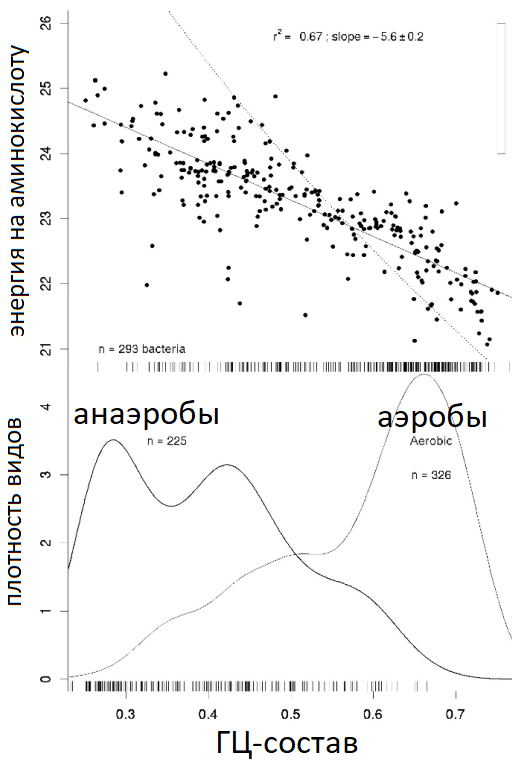
\includegraphics [width=0.5\textwidth] {Dissertation/images/lit/lit1.png}
  \caption{Аэробные бактерии имеют более высокий ГЦ-состав и используют аминокислоты, требующие меньше энергозатрат для синтеза в аэробных условиях. График сверху: зависимость средней энергии, которую нужно затратить на синтез аминокислот представленных в протеоме бактерий, от ГЦ-состава. График снизу: плотность распределения ГЦ-состава у аэробных и анаэробных микроорганизмов. Источник изображения: \cite{lobry2004life}.} 
  \label{img:gc1}  
\end{figure}

Анализ лабораторных экспериментов по накоплению мутаций выявил значительное мутационное смещение в сторону увеличения ГЦ-состава \cite{long2018evolutionary}. Причем оно наблюдалось как в четырежды вырожденных сайтах (все замены являются синонимичными), так и в ноль-вырожденных сайтах (все замены являются несинонимичными), хотя в последних и в значительно меньшей степени. 

\subsection{ГЦ смещение генома}
Неравномерная представленность нуклеотидов в лидирующей и отстающей цепи была обнаружена в 60-х годах двадцатого века \cite{szybalski1966pyrimidine}. Анализ первых трех секвенированных геномов показал, что лидирующая цепь почти равномерно обогащена нуклеотидами Г и Т, в то время как в отстающей чаще встречаются A и Ц \cite{lobry1996asymmetric}. Позднее, данная закономерность, названная ГЦ смещением (GC skew) была выявлена у эубактерий и архей, геномов митохондрий, хлоропластов и вирусов, но не для эукариот со множественными сайтами инициации репликации \cite{lobry1999genomic}. Существуют бактерии без выраженного ГЦ смещения, например, некоторые цианобактерии: \textit{Gloeobacter violaceus} и \textit{Synechococcus elongatus} \cite{arakawa2007gc}. Основную роль в возникновении ГЦ смещения играет, по-видимому, различная мутационная нагрузка на две цепи ДНК, действующая во время репликации. При репликации, лидирующая и отстающая (достраивающейся за счет фрагментов Оказаки) цепи проводят неравное время в одноцепочечном состоянии и в различной степени подвержены дезаминированию, с последующей заменой цитозиновых нуклеотидов на тиминовые. Данные в пользу этого предположения были получены в лабораторных экспериментах по ускоренной эволюции, в которых было показано влияние уровня дезаминирования цитозина (которое, контролировалось в эксперименте) на итоговый уровень ГЦ смещения \cite{kono2018accelerated}. 

\subsection{Chi сайты неравномерно расположены в геноме}
Для сохранения жизни необходима стабильность генома. Для колонизации новых экологических ниш, борьбы с конкурентами, создания более высокоорганизованных организмов, наоборот, нужна динамичность генома - возможность появления и сохранения изменений. Как в обеспечении постоянства генома, так и в его изменчивости, важную роль играет процесс рекомбинации - обмен молекул ДНК своими фрагментами.

Хорошо изучен процесс гомологичной рекомбинации, под которой понимают процесс образования контакта между идентичными или схожими по последовательности фрагментами ДНК с последующим обменом генетическим материалом. Данный процесс позволяет клеткам восстанавливать поврежденные участки ДНК, при условии наличия неповрежденной копии \cite{kuzminov1999recombinational}. Гомологичная рекомбинация также задействована в возобновлении работы остановившихся вилок репликации (например, в следствии недостаточно эффективной работы хеликазы, слишком высокой скрученности ДНК в области репликации, значительного количества белков связанных с ДНК, столкновении репликазы и РНК полимеразы \cite{michel2000resolution, sankar2016nature}.

У прокариот гомологичная рекомбинация играет большую роль в пластичности генома. Именно благодаря этому процессу осуществляются дупликации либо делеции участков ДНК при репликации либо транскрипции, а также замена фрагментов генома на чужеродный материал при горизонтальном перенос генов \cite{ochman2000lateral}. 

В случае, когда в рекомбинации участвуют чужеродные фрагменты ДНК, выделяют два возможных исхода (рисунок~\ref{img:dco_sco}). В одном случае, у двух фрагментов имеются схожие последовательности на краях, и в результате один фрагмент заменяется на другой (рисунок~\ref{img:dco_sco}). Если же привходящая ДНК находится в кольцевой форме и обладает одним схожим по последовательности фрагментом, то происходит вставка без вырезания. 

\begin{figure}[!ht] 
  \center
    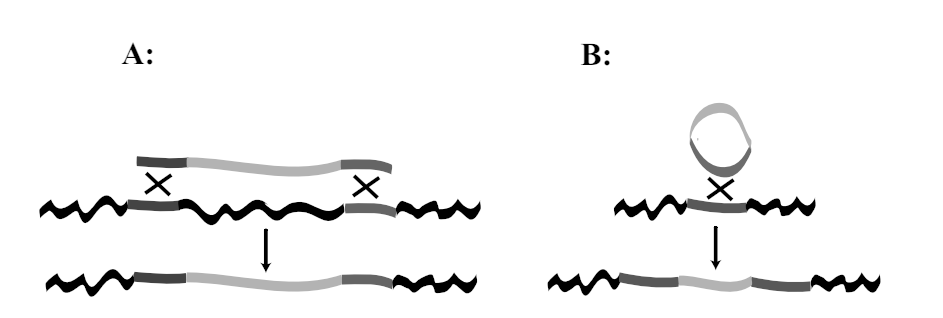
\includegraphics [width=0.75\textwidth] {Dissertation/images/lit/recombination/recombination_dco_sco.png}
    \caption{Варианты рекомбинации при участии чужеродного фрагмента ДНК. Схожие по последовательности фрагменты обозначены темно-серым цветом. А: в случае наличия схожих фрагментов на краях молекул, одна последовательность заменяется на другую; В: в случае, когда привходящая ДНК находится в кольцевой форме и обладает одним участком с высоким сходством последовательности, происходит вставка нового материала без потери исходного варианта. Источник изображения: \cite{mullany2005dynamic}.}
    \label{img:dco_sco}
\end{figure}

У бактерий процесс рекомбинации хорошо изучен на примере кишечной палочки \textit{E. coli}. Важную роль в рекомбинации у данного организма играет комплекс белков RecВCD, обладающий хеликазной, экзо- и эндонуклеазной активностями. Работа этих белков создает ДНК с "липким"\ концом - краевым одноцепочечным фрагментом, что является необходимым условием дальнейших этапов рекомбинации. 

Для образования липких концов необходимо наличие несимметричного разрыва двухцепочечной ДНК. При этом липкие концы образуются на некотором расстоянии от места разрыва. Это расстояние определяется локализацией специфичных последовательностей - Chi сайтов. Данные сайты распознаются белками комплекса RecBCD и, в зависимости от соотношения концентрации АТФ и ионов магния, происходит либо надрез цепи в зоне Chi сайта, либо завершается экзонуклеазная активность RecBCD комплекса (рисунок~\ref{img:rec_chi}) \cite{smith2012recbcd, singleton2004crystal}. В дальнейшем, на одноцепочечном фрагменте происходит кластеризация белка RecA, образование синапса, переброс цепей, образование и разрешение структуры Холидея. 

\begin{figure}[!ht] 
  \center
    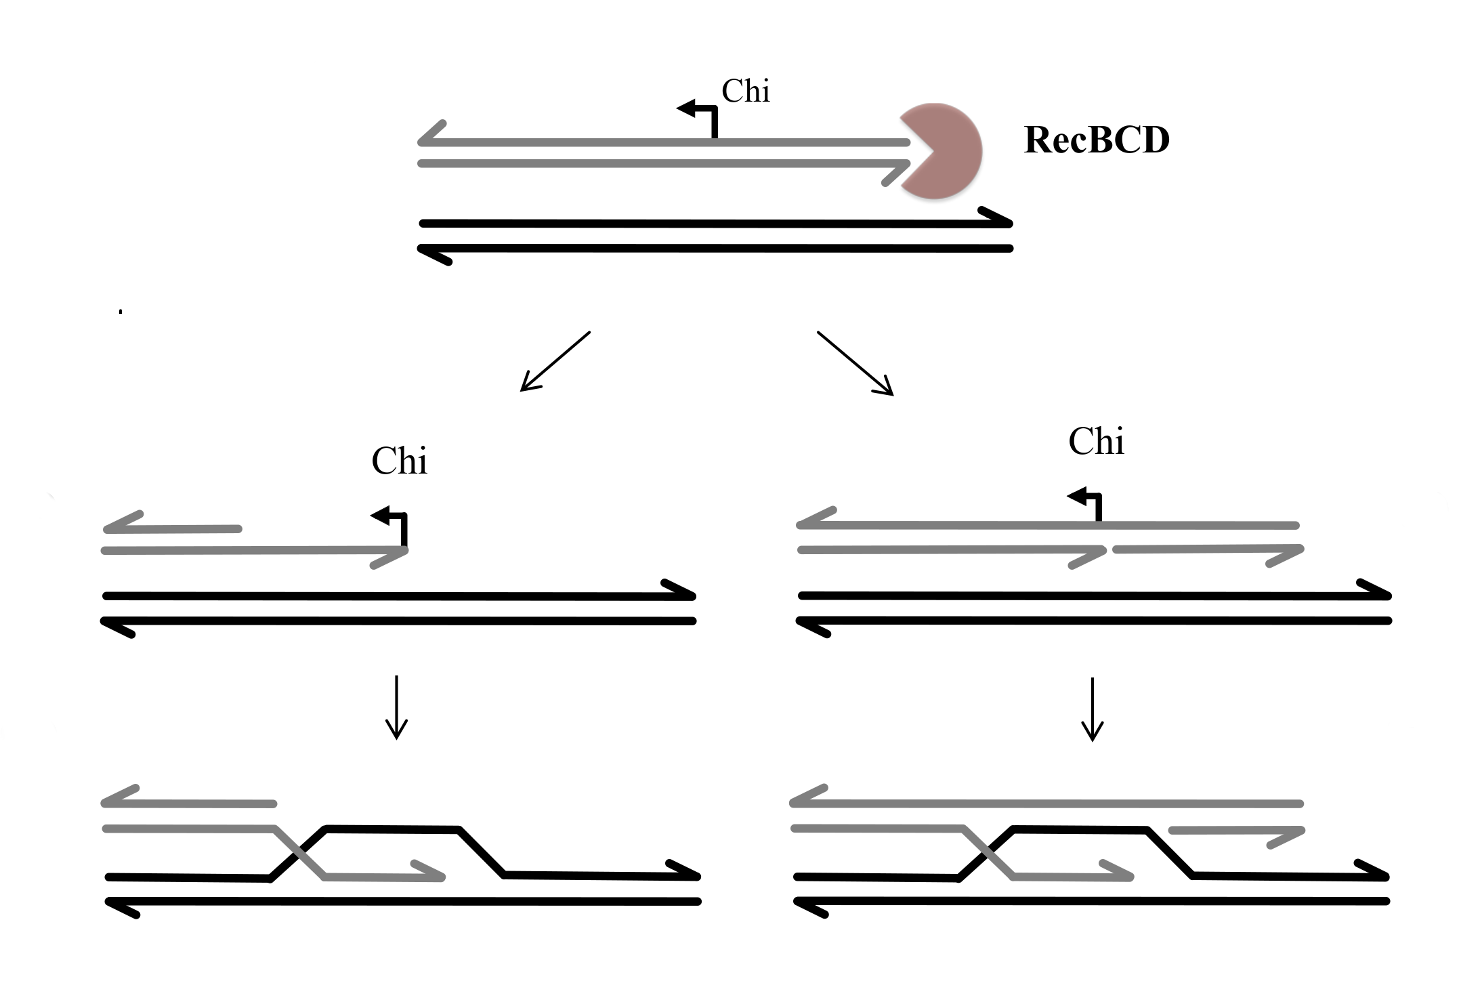
\includegraphics [width=0.85\textwidth] {Dissertation/images/lit/recombination/recombination_chi.png}
    \caption{Участие Chi сайтов в процесса рекомбинации. Данная последовательность распознается белками RecBCD комплекса, что приводит к прекращению продвижения комплекса вдоль цепи ДНК и задает локализацию двухцепочечного разрыва. Источник изображения: \cite{azeroglu2016recg}.}
    \label{img:rec_chi}
\end{figure}

Название сайта Chi является сокращением от crossover hot spot instigator (инициатор горячих точек перекреста). Данные сайты были обнаружены как последовательность, необходимая для осуществления RecBCD зависимой рекомбинации фага лямбда \cite{lam1974rec}. В геноме \textit{E. coli}, находится около тысячи Chi сайтов (примерно по одному на 5 тысяч п.н.) \cite{malone1978hotspots}.

Chi сайты распределены в геноме не равномерно. Они представлены преимущественно в общей для вида части генома, в кор-геноме (core-genome), что вероятно способствует поддержанию его стабильности \cite{halpern2007identification}. В то же время, рибосомные опероны не содержат в себе Chi сайтов (но содержали бы при их случайном расположении) \cite{reams2014recombination}. Наблюдается более редкая встречаемость Chi сайтов в повторяющихся участках генома, что, по-видимому, защищает геном от лишних перестроек, которые бы возникали в случае близкорасположенных повторов \cite{li2019positioning}.

\subsection{Пространственная укладка генетического материала}
У всех организмов ДНК находится в свернутом состоянии, что необходимо для ее размещения внутри клетки (длина хромосомы на несколько порядков превышает длину клетки) \cite{dame2020chromosome}. При этом, пространственная конфигурация молекулы ДНК не случайна, она отражает и регулирует функциональное состояние генома \cite{dekker2008gene}. Так, для эукариот было показано, что петли хроматина, которые размещают промоторы и удаленные энхансеры в непосредственной пространственной близости, играют важную роль в регуляции транскрипции \cite{vernimmen2007long}. У прокариот, укладка хромосомы также, по-видимому, неслучайна и выполняет ряд функций \cite{hofmann2015role}. Подходы, основанные на флуоресцентной микроскопии, позволяют определять субклеточное положение отдельных хромосомных локусов, а высокопроизводительные подходы на основе методов 3C и Hi-C позволяют количественно определять частоты взаимодействия между локусами, которые впоследствии могут использоваться для определения средних трехмерных расстояний между ними. Автоматизация этих методов в начале 2000-х годов позволила проводить исследования пространственной укладки хромосом в масштабе всего генома \cite{umbarger2011three}. 
 
Укладка хромосом у прокариот имеет иерархический характер: от крупномасштабных макродоменов до более мелких структур. Она контролируется при помощи нуклеоид-ассоциированных белков \cite{dame2020chromosome}, одним из которых является гистоноподобный белок H-NS. Он прикрепляется к ДНК преимущественно в локусах с повышенным AT составом и высокой частотой ApT динуклеотида, что характерно для горизонтально перенесенных фрагментов генома \cite{lucchini2006h}. Склонность белка H-NS к образованию цепочек стимулирует образование протяженных нуклеопротеиновых филаментов вдоль одной либо между двух спиралей ДНК \cite{dame2006bacterial}. Считается, что у \textit{E. coli} основными функциями данного белка являются компактизация ДНК и снижение уровня экспрессии горизонтально перенесенных генов \cite{dame2020chromosome}. Множество бактерий имеют гомологи, либо аналоги белка H-NS.

 Другим важным способом поддержания пространственной укладки ДНК являются комплексы структурного поддержания хромосом (structural maintenance of chromosomes, SMC). Эти комплексы способствуют образованию петель ДНК и поддерживают их устойчивость, формируя кольцеобразную структуру вокруг петель \cite{nolivos2014bacterial}. Комплексы SMC также участвуют в сегрегации вновь реплицированных сестринских хромосом \cite{dame2020chromosome}. Мутанты \textit{E. coli} по гену mukB (один из основных белков SMC комплекса у данного организма) имеют нарушенное разделение ДНК по дочерним клеткам и часто производят клетки, лишенные хромосомы \cite{hiraga1989chromosome}. Ряд других белков (IHF, HU, Fis) участвуют в формировании пространственной укладки за счет изгибания ДНК и поддержания её отрицательной суперскрученности \cite{dame2020chromosome}. 

В масштабе от десятков до сотен тысяч оснований, бактериальная хромосома разделена на домены взаимодействия хромосом (chromosome interaction domains, CID), которые аналогичны топологически ассоциированным доменам (topologically associating domains, TAD) у эукариот. ДНК расположена значительно ближе и чаще контактирует внутри доменов, чем между ними (рисунок~\ref{img:chr3d}) \cite{dame2020chromosome}. 

\begin{figure}[!ht] 
  \center
  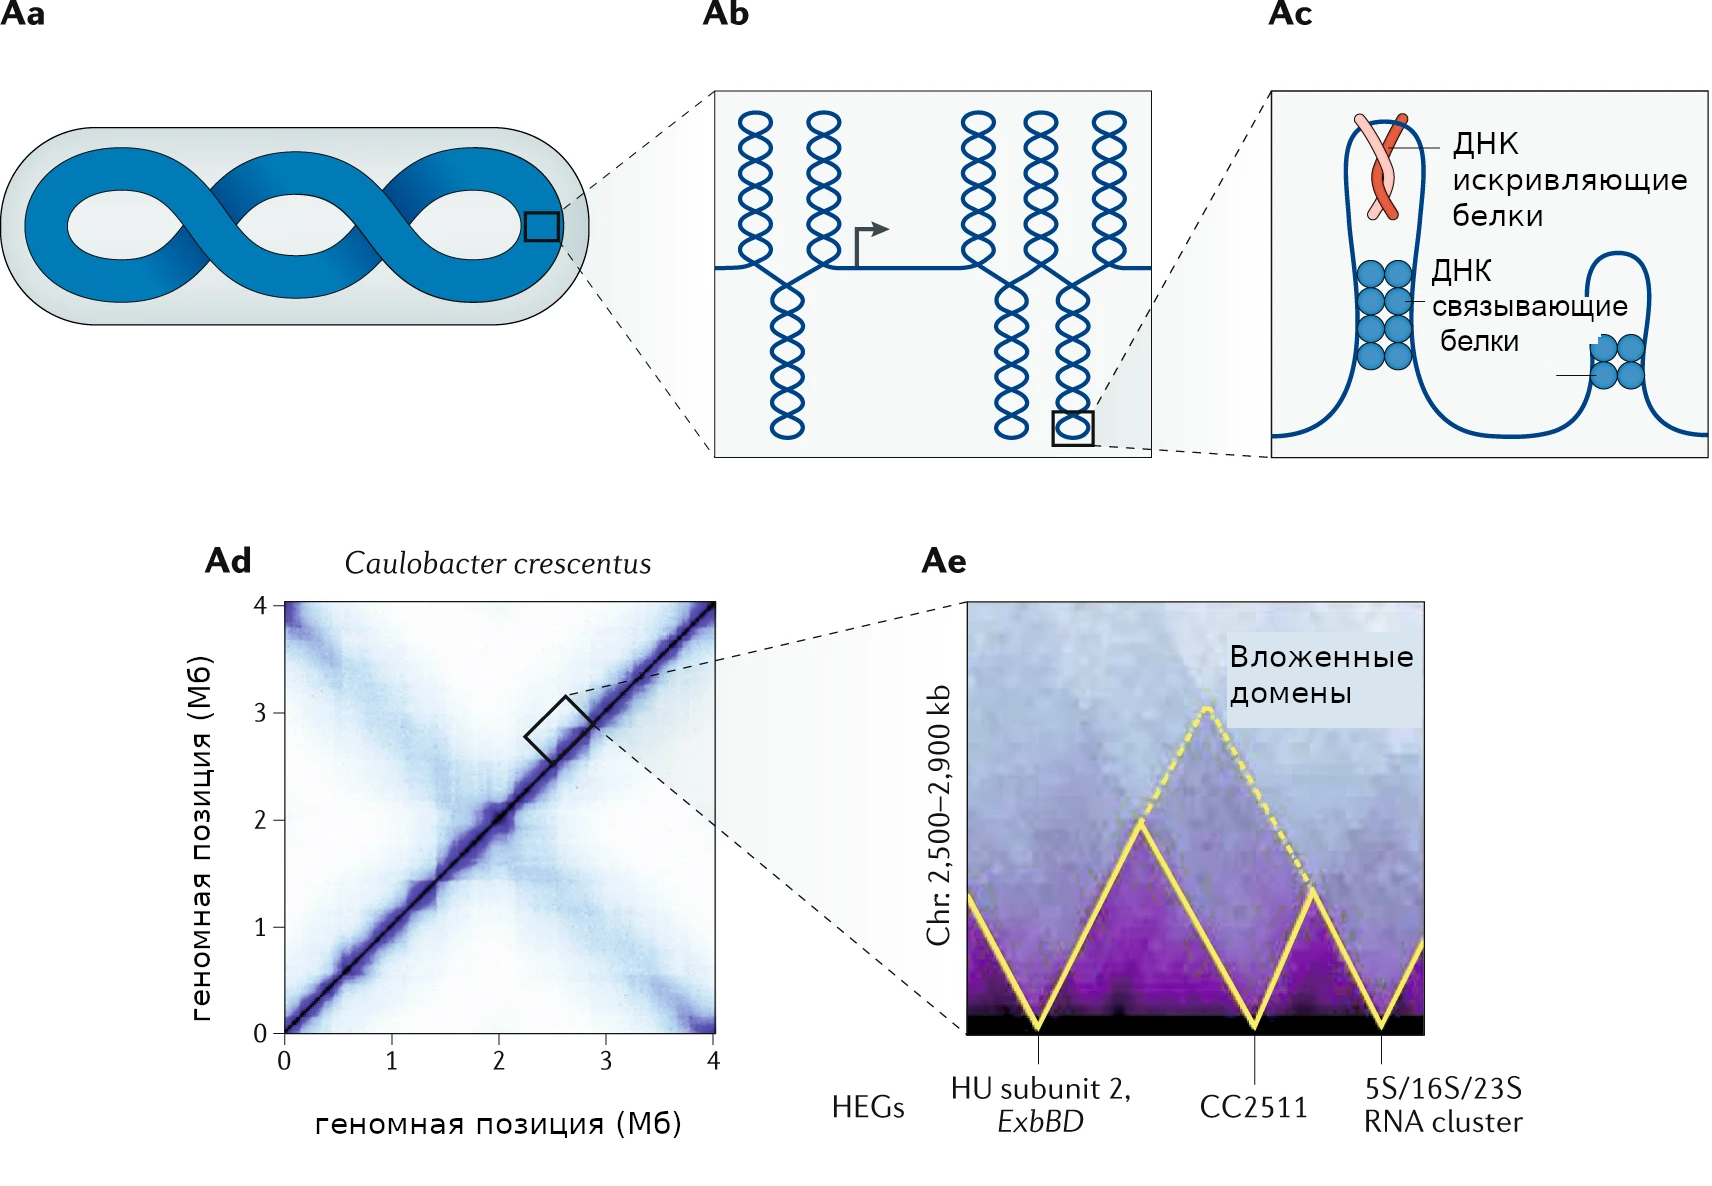
\includegraphics [width=0.9\textwidth] {Dissertation/images/lit/chromosome3d_1.png}
  \caption{Уровни организации пространственной укладки ДНК у прокариот. Пространственная укладка хромосомы многих бактерий имеет форму спирали (Aa), что выражается в наличии двух диагоналей на карте хромосомных контактов (Ad). В масштабе от десятков до сотен тысяч оснований хромосома подразделяется на домены взаимодействия хромосом (Ab). Эти структуры выглядят как квадраты вдоль главной диагонали карты хромосомных контактов (Ad) или как треугольники при наблюдении одной половины симметричной карты(Ae). Домены взаимодействия часто являются вложенными: более крупные домены (прерывистая желтая линия) организованы в более мелкие субдомены (сплошная желтая линия) (Ae). Границы между доменами обычно образованы высокоэкспрессируемыми генами длиной более 2 т.п.н., которые физически разделяют фланкирующий хроматин (часть Ab). Изображение адаптировано из \cite{dame2020chromosome}.} 
  \label{img:chr3d}  
\end{figure}

Количество доменов может зависеть от состояния клетки, так у \textit{Caulobacter crescentus} хромосома организована в 23 домена взаимодействия во время экспоненциального роста в богатой среде и в 29 доменов в условиях голодания; изменение количества доменов вероятно связано с изменением уровня транскрипции генов \cite{dame2020chromosome}. В хромосоме \textit{E. coli} можно выделить 31 домен взаимодействия размером от 40 до 300 тысяч п.н. Двадцать две границы домена соответствуют положениям высоко экспрессируемых генов, а девять границ совпадают с положениями генов, кодирующих белки с сигнальной последовательностью экспорта \cite{lioy2018multiscale}. Выделенное положение генов, кодирующих экспортируемые из клетки белки, может объясняться необходимостью сопряжения процессов транскрипции, трансляции и транслокации \cite{woldringh2002role}. Бактериальные домены взаимодействия имеют вложенный (иерархический) характер, каждый домен состоит из меньших субдоменов (рисунок~\ref{img:coli_3d} Ae), самые мелкие единицы этой организации могут соответствовать отдельным оперонам \cite{dame2020chromosome}.

\begin{figure}[!ht] 
  \center
  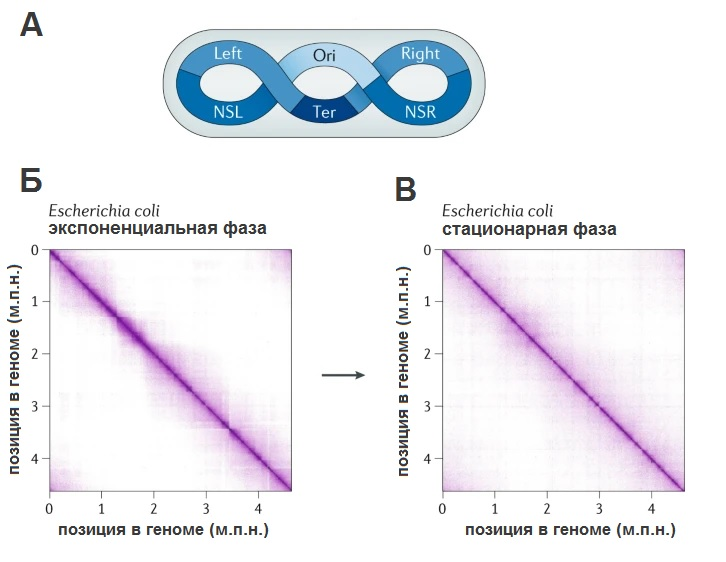
\includegraphics [width=0.9\textwidth] {Dissertation/images/lit/coli_3d.jpg}
  \caption{Пространственная укладка хромосомы \textit{E. coli}. А) Схематическое изображение пространственной укладки хромосомы \textit{E. coli}, в которой выделяют следующие макродомены: левый (Left), правый (Right), макродомен около сайта начала репликации (Ori) и места окончания репликации (Ter). Б) карта межхромосомных контактов в экспоненциальной фазе роста. В) карта межхромосомных контактов в стационарной фазе роста. Изображение адаптировано из \cite{dame2020chromosome}.} 
  \label{img:coli_3d}  
\end{figure}


Наиболее крупным уровнем пространственной организации прокариотической хромосомы являются макродомены. У \textit{E. coli} хромосома разделена на четыре макродомена и две неструктурированные области (рисунок~\ref{img:coli_3d} ). Все макродомены обладают пониженной подвижность внутри клетки по сравнению с неструктурированными хромосомными участками. Таким образом, макродомены имеют тенденцию взаимодействовать с неструктурированными областями, но не с другими макродоменами \cite{espeli2008dna}. У \textit{E. coli} выделяют макродомен около сайта начала репликации (Ori домен). Ограниченная подвижность Ori домена требует активности белка MaoP (белок макродомена Ori) и мотива из 17 нуклеотидов в вышележащей межгенной области, названной maoS (последовательность макродомена Ori) \cite{valens2016maop}. Механизм, благодаря которому белок MaoP ограничивает подвижность ДНК остается не известен \cite{dame2020chromosome}. Макродомен Ter содержит место окончания репликации, для него описан белок MatP (macrodomain Ter protein), необходимый для существования макродомена (при деактивации данного белка ДНК становится неструктурированной). Белок MatP распознает мотив из 12 нуклеотидов, встречающийся преимущественно в Ter регионе. 

Макродоменная организация хромосомы более выражена во время экспоненциальной фазы роста бактерий. Переход к стационарной фазе связан со снижением уровня доменной организации ДНК, что наблюдается как "размытие"\ квадратов, соответствующих доменам, на карте межхромосомных контактов, получаемой в экспериментах на основе метода HI-C \cite{lioy2018multiscale}.

\section{Горизонтальный перенос генов}
Бактерии и археи размножаются в основном за счет бинарного деления, которому предшествует дупликация генома в родительской клетке. Дочерние клетки получают геном от родительской клетки, что называется вертикальным наследованием. Существует процесс горизонтального переноса генов (ГПГ), при котором клетки приобретают чужеродный генетический материал. На основе анализа геномов было установлено, что горизонтальный перенос часто встречается у прокариот и вероятно сыграл важную роль в их эволюции. Данный процесс позволяет микробам приобретать новые метаболические возможности, занимать новые экологические ниши, приобретать резистентность к воздействию антибиотиков, фагов, атак со стороны эукариот \cite{ochman2000lateral, rodriguez2016flexible, niehus2015migration}. Горизонтальный перенос генов внес наибольший вклад в расширение генных семейств (появления различных вариантов гомологичных белков) \cite{treangen2011horizontal}. В настоящее время интерес к этому процессу во многом продиктован ростом числа резистентных к антибиотикам бактерий, в том числе, бактерий устойчивых ко всем известным антибиотикам \cite{sun2019horizontal}. 

Горизонтальный перенос генов происходит наиболее часто между близкородственными организмами, что объясняется наличием барьеров для переноса между филогенетически-далекими организмами и зачастую низкой функциональностью генов, приобретенных от несхожих организмов \cite{gonzalez2012barriers}. Тем не менее, описаны случаи переноса крупных фрагментов генома между дальнородственными организмами \cite{caro2015inter}. Например, у архей часто находят гены, горизонтально перенесенные от бактерий \cite{wagner2017mechanisms}. В недавней работе, был сделан вывод о происхождении гетеротрофных аэробных архей haloarcheae от архей, являющихся аутотрофными анаэробами, в результате переноса большого фрагмента бактериальной ДНК, содержащей около 1000 генов \cite{wagner2017mechanisms}. Описаны отдельные случаи переноса генов между про- и эукариотами \cite{lacroix2016transfer}. 

Основные способы горизонтального переноса генов у бактерий и архей таковы: трансдукция --- перенос генов при помощи фагов, трансформация --- захват ДНК из окружающей среды, конъюгация --- проникновение ДНК от клетки-донора при контакте с клеткой-реципиентом \cite{thomas2005mechanisms, wagner2017mechanisms}. Описаны и более экзотические способы, при помощи ДНК содержащих мембранных везикул \cite{biller2014bacterial}, передача ДНК при контакте бактерий с помощью синтезируемых ими нанотрубок \cite{dubey2011intercellular}, вирусоподобные агенты горизонтального переноса (virus-like gene transfer agents, GTA) \cite{brimacombe2015homologues}. В большинстве типов переноса, переносимая ДНК должна находиться в одноцепочечной форме, у \textit{E. coli} также описаны механизмы переноса двухцепочечной ДНК \cite{sun2018pull}.

\subsection{Трансформация}
Трансформация --- это процесс захвата и интеграции внеклеточной ДНК характерный для прокариот. Поглощение ДНК требует, чтобы клетка находилась в физиологическом состоянии, известном как компетентность. Для поддержания состояния компетентности требуется активность нескольких десятков (20–50) белков, которые как правило высоко-консервативны \cite{thomas2005mechanisms, sun2018pull}. Интенсивность трансформации зависит от ряда факторов: от концентрации внеклеточной ДНК, от количества соседних компетентных клеток, степени нехватки ресурсов (стресса) \cite{johnston2014bacterial}. 

При трансформации, перемещаемая  ДНК становится одноцепочечной при прохождении через мембрану, и затем может подвергаться гомологичной рекомбинации или использоваться в качестве источника питательных веществ \cite{finkel2001dna}. Интересно, что в то время как белки участвующие в транслокации ДНК обладают высокой консервативностью (почти у всех видов эту функцию выполняют гомологичные белки), пути, регулирующие переключение в состояние компетентности, значительно различаются - у разных видов в этом участвуют различные белки, реагирующие на различные сигналы \cite{johnston2014bacterial}. Это значительно усложняет определение того, является ли некоторый вид естественно-компетентным. Так, \textit{Vibrio cholerae} не считался компетентным до обнаружения роли продуктов распада хитина в индукции состояния компетентности \cite{mell2014natural}. У некоторых видов (например, различных видов \textit{Neisseria} и \textit{Helicobacter}) клетки находятся в компетентном состоянии почти все время жизни \cite{dubnau2019mechanisms}.

Захват ДНК в бактериальных клетках осуществляется при помощи пилей IV типа либо иными подобными структуры \cite{piepenbrink2019dna}. Этот процесс наиболее хорошо изучен у грамм-отрицательных бактерий, в частности у \textit{Vibrio cholerae} и \textit{Neisseria gonorrhoeae}. У данных бактерий после захвата ДНК, пиль сокращается, ДНК проникает внутрь клетки, после чего связывается с периплазматическими белками для предотвращения обратной диффузии, одна цепь ДНК затем переносится через цитоплазматическую мембрану, а другая цепь деградирует \cite{dubnau2019mechanisms}. Подобный механизм, вероятно,
действует и у грамположительных бактерий, но эти системы изучены в меньшей степени \cite{dubnau2019mechanisms}.

\subsection{Мобильные элементы генома}
Горизонтальный перенос генов часто осуществляется при участии мобильных элементов генома. Под мобильными элементами генома понимают фрагменты ДНК, которые способны перемещаться внутри генома или между геномами различных клеток и кодируют все либо часть белков, необходимых для своего перемещения \cite{bellanger2014conjugative}. Наиболее известными и хорошо изученными мобильными элементами являются плазмиды, траспозоны и бактериофаги. Ниже приведено короткое описание этих и некоторых других типов мобильных элементов. 
%https://www.sciencedirect.com/science/article/abs/pii/S1369527416301801

\subsubsection{Плазмиды}
Плазмиды --- это кольцевые или линейные внехромосомные репликоны, которые присутствуют во многих бактериях и археях и встречаются у эукариот \cite{shintani2015genomics}. Они являются одним из основных средств обмена генетической информацией у микробов благодаря способности эффективно перемещаться из одного организма в другой при помощи конъюгации \cite{guglielmini2011repertoire}. 

Длина плазмид находится в диапазоне от единиц до сотен тысяч пар нуклеотидов. Их репликация может осуществляться различными способами. Для кольцевых плазмид характерна тета-репликация, репликация по типу "катящегося кольца", репликация с вытеснением цепи \cite{del1998replication}. На краях линейных плазмид, как правило, присутствуют короткие повторы по функциям схожие с теломерами, которые играют важную роль в репликации данных плазмид \cite{ravin2011n15}.

Конъюгативные плазмиды несут в себе генетически сложные системы для горизонтальной передачи плазмид, включая белки для образования пор спаривания, а также белки репликации и передачи ДНК. Существуют мобилизуемые плазмиды, которые кодируют только часть функций, необходимых для переноса; их горизонтальная передача может происходить только при наличии в клетки других плазмид, несущих недостающие белки. Соотношение подвижных плазмид (коньюгативных и мобилизуемых) к плазмидам, для которых не обнаружены факторы передачи (немобильные), равно примерно 2:1 \cite{redondo2020pathways}. Немобильные плазмиды также могут горизонтально передаваться при помощи процесса трансформации \cite{hulter2017evolutionary}. 

Недавний анализ более чем десяти тысяч плазмид, показал, что для них можно выделить кластеры ("таксономические единицы") с высоким сходством последовательностей внутри кластеров (выше 90\%) и низким, как правило, ниже 70\% сходства в остальных случаях \cite{redondo2020pathways}.

Плазмиды могут встраиваться в хромосому своих хозяев и таким образом обеспечивать изменчивость хромосом \cite{zechner2000conjugative, brunder2000genome}. Такие интеграционные события были обнаружены в геномах \textit{Enterococcus faecalis}, \textit{Shigella flexneri}, \textit{Yersinia pestis}, \textit{E. coli} и ряда других организмов \cite{myers2006role}. 

Встраивание плазмид может сильно влиять на фенотип организма. Для \textit{S. flexneri} и \textit{E. coli} описана плазмида размером 220 т.п.н., встраивание которой в хромосому приводит к тому, что факторы вирулентности, кодируемые данной плазмидой, перестают экспрессироваться и бактерии теряют способность к инвазии. Затем может произойти точное вырезание плазмиды, с восстановлением вирулентности бактерии. Также может происходить неточное (частичное) вырезание, что может приводить к тому, что фрагменты плазмиды остаются в хромосоме \cite{myers2006role}. Описан ретро-транспорт плазмид --- их передача в клетку-рецепиент с последующим возвратом в донорскую клетку. Данный процесс может служить способом приобретения новых генов клеткой-донором, за счет их встраивания в плазмиду, при ее нахождении в клетке-реципиенте \cite{ronchel2000retrotransfer}. Плазмиды обладают высоким уровнем изменчивости и часто содержат в себе различные мобильные элементы. Конъюгативные и мобилизуемые плазмиды таким образом могут служить средством транспорта мобильных элементов генома от одних клеток к другим. Интересной и сравнительно новой темой исследований является взаимосвязь мобильных элементов генома. Так, для холерного вибриона описана мобилизация геномного острова конъюгативной плазмодой \cite{carraro2016inca}. Согласно предложенной модели, мобилизация обеспечивается тем, что на плазмиде кодируется транскрипционный фактор AcaCD, который активирует в том числе и гены, находящиеся в геномных островах, в частности ген фактора направленности рекомбинации xis, продукт которого увеличивает частоту вырезания геномного острова из хромосомы \cite{carraro2017mobilizable}. 

\subsubsection{Интегративные конъюгативные элементы}
Впервые, процесс конъюгации был открыт на плазмидах \cite{lederberg1946gene}. Позднее были обнаружены хромосомные элементы генома способные к вырезанию и конъюгативной передаче --- интегративные конъгативные элементы (ИКЭ)\cite{burrus2002icest1}. Вырезание и интеграция ИКЭ осуществляется за счет интеграз либо транспозаз. На рисунке~\ref{img:ice} показано схематичное изображение структуры и принципа функционирования интегративных конъюгативных элементов. 

\begin{figure}[!ht] 
  \center
  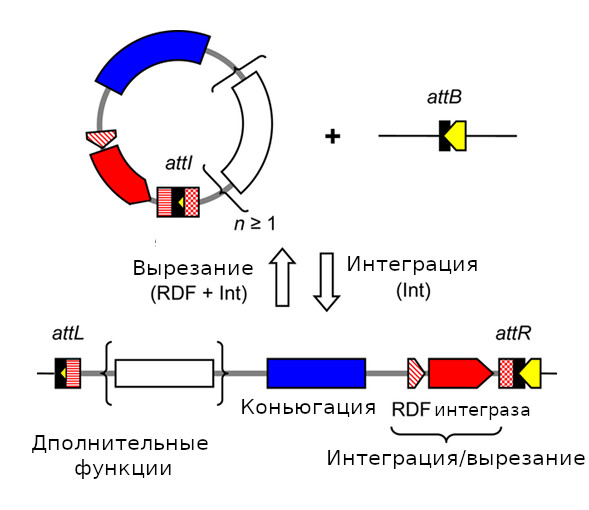
\includegraphics [width=0.7\textwidth] {Dissertation/images/lit/ice.jpg}
  \caption{Устройство и принцип работы интегративных конъюгативных элементов (ИКЭ). Сайт-специфическая интеграция и вырезание катализируются интегразой. RDF является кофактором, необходимым для процесса вырезания (у ряда интеграз). Большие прямоугольники обозначают модули. Тонкие черные линии и толстые серые линии обозначают геном хозяина и ИКЭ, соответственно. Стрелками обозначены гены, а меленькими прямоугольниками - сайты интеграции. Изображение адаптировано из \cite{bellanger2014conjugative}.} 
  \label{img:ice}  
\end{figure}

Разные типы интеграз и транспозаз отличаются сайтами интеграции и уровнем сайт-специфичности. Наиболее хорошо изучены ИКЭ, кодирующие тирозиновые рекомбиназы. Они часто обладают высокой сайт специфичностью, а сайты интеграции широко представлены в генах тРНК и ряде других генов домашнего хозяйства. Описаны также ИКЭ с низкой сайт-специфичностью интеграции. Например, элемент CTnDOT, встречающийся у бактерий рода \textit{Bacteroides} и встраивается в низко-специфичные (но не случайные) сайты \cite{cheng2000integration}. 

Интегративные конъюгативные элементы, наряду с плазмидами, считаются одними из наиболее эффективных способов распространения генов устойчивости к антибиотикам \cite{botelho2020role}. ИКЭ семейства SXT были признаны основными факторами распространения генов устойчивости к антибиотикам среди нескольких видов семейств Enterobacteriaceae и Vibrionaceae, включая экологические и клинические изоляты \textit{V. cholerae} \cite{carraro2015biology}. 

Интегративные конъюгативные элементы значительно отличаются по длине: от десятков т.п.н. (например, элемент pSAM2 у \textit{Streptomyces ambofaciens} \cite{pernodet1984plasmids}) то сотен т.п.н. (у \textit{Streptomyces turgidiscabies} описан элемент PAISt длиной в 674 т.п.н.\cite{kers2005large}). Эта разница в размере в значительной степени зависит от карго-генов, количество которых варьирует от одного гена устойчивости к тетрациклину у Tn916 (одного из наиболее хорошо изученных ИКЭ), до значительного числа генов (в том числе с неизвестными функциями) у PAISt. Состав карго-генов может значительно между близкими ИКЭ, несущими одинаковые либо схожие по последовательности модули конъюгации и рекомбинации. 

\subsubsection{Фаги}
Фаги - вирусы бактерий и архей - являются важным фактором изменчивости геномов своих хозяев \cite{ventura2002transcription}. Первые проекты по секвенированию бактериальных геномов показали значительный вклад профаговых последовательностей в наблюдаемые межштаммовые отличия. Так, в последовательности генома \textit{E. coli O157 Sakai} было идентифицировано 18 профагов (или остатков профагов), они составили примерно половину всех различий в генном составе между данным штаммом и лабораторным \textit{K-12} \cite{hayashi2001complete}. 


Размеры фаговых геномов значительно варьируют, наименьший описанный фаговый геном состоит всего из 2,4 т.п.н., а размеры наиболее длинных геномов превышают 400 т.п.н. Подобно остальным мобильным элементам, фаговые геномы могут нести карго-гены, среди которых встречаются гены патогенности (включая, токсины) \cite{schroven2021bacteriophages}. Так, некоторые фаги семейства лямбда содержат в себе шига-токсин, который является мощным фактором патогенности у шига-продуцирующих \textit {E. coli}; у \textit{Vibrio cholerae} описаны нитчатые фаги CTXf, несущие ген, кодирующий токсин холеры (CTX); известны фаги, наличие которых необходимо для патогенности бактерий \textit{Corynebacterium diphtheriae} и \textit{Clostridium botulinum} \cite{brussow2004phages}. Ряд факторов патогенности присутствует в фагах золотистого стафилококка, сальмонелл, стрептокков \cite{brussow2004phages}. Экспериментально было показано, что некоторые гены вирулентности, содержащиеся в фагах, могут экспрессироваться при нахождении его в виде профага \cite{ventura2002transcription}, ряд других генов (например, шига-токсин фагов семейства лямбда) экспрессируются только когда фаг находится в литической фазе цикла \cite{berger2019carriage}.

Фаги могут участвовать в горизонтальном переносе генов у своих хозяев при помощи процессов специальной и общей (генерализованной) трансдукции \cite{canchaya2003phage, touchon2017embracing}. Умеренные фаги могут встраиваться в геном хозяина - становиться профагами. При последующей индукции, происходит вырезание профага из генома хозяина и наработка вирусных частиц, с последующим их выходом из клетки. Вырезание профага может не совпадать с границами вирусной последовательности и содержать соседние области генома. Тогда части ДНК клетки-хозяина попадут в капсид и будут перенесены в новую клетку, заражаемую фагом. Данный процесс называется специализированной трансдукцией. В соответствии с этой моделью, в ряде геномов в непосредственной близости от сайта интеграции фагов обнаруживаются горизонтально перенесенные гены \cite{canchaya2003phage}. 

Хорошо изучен механизм интеграции у фага лямбда. Интеграза данного фага представляет собой сайт-специфическую тирозиновую рекомбиназу, обеспечивающую рекомбинацию между двумя комплементарными последовательностями ДНК: сайтом attP (250 п.н.), расположенный в геноме фага, и сайте attB (21 п.н.), расположенном внутри бактериального генома \cite{mohaisen2020site}. У многих других фагов, использующих сайт-специфическую рекомбинацию, для успешной интеграции необходимо наличие вспомогательных белков --- факторов интеграции, кодируемых бактериями \cite{mohaisen2020site}. 


Горизонтальный перенос генов может происходить также за счет общей (генерализованной) трансдукции, при которой ДНК хозяина упаковывается в капсид вместо генетического материала фага. После заражения другой клетки, такая ДНК может участвовать в процессе рекомбинации и стать частью генома зараженной клетки. У некоторых бактерий, фаги являются механизмом передачи определенных, неслучайных, фрагментов ДНК. Так, у \textit{Staphylococcus aureus} описан остров патогенности SaPI1 длиной 15 т.п.н., кодирующий токсин Tst участвующий в токсическом шоке. В клетках стафилококка, инфицированных фагом 80a, этот остров вырезается из хромосомы, автономно реплицируется и попадает в капсид собираемых фагов. При проникновении в организм-реципиент, SaPI1 интегрируется с использованием собственных интеграз \cite{ruzin2001molecular}. 

Фаговые геномы обладают высоким уровнем изменчивости, а их отдельные фрагменты часто имеют различную эволюционную историю (мозаицизм) \cite{hatfull2011bacteriophages}. Вероятно, основным фактором такой изменчивости, является незаконная рекомбинация или рекомбинация между короткими консервативными последовательностями; значительный вклад в эти процессы могут вносить фаговые рекомбиназы \cite{hendrix2000origins, hatfull2011bacteriophages}. Особенностью горизонтальной передачи генов при помощи фагов является их устойчивость: фаги могут сохранять свою способность к инфицированию на протяжении многих лет, даже в агрессивной внешней среде, в которой свободная ДНК деградирует. Фаги, как правило, обладают более узким спектром хозяев (по сравнению с плазмидами), что вероятно объясняется их зависимостью от наличия специфических рецепторов на инфицируемых клетках \cite{myers2006role}.
% https://www.sciencedirect.com/science/article/pii/S1369527403000869

\subsubsection{Интегроны}
Интегроны --- это специализированные системы приобретения генов в бактериальных геномах \cite{gillings2014integrons}. Они достаточно широко распространены и встречаются примерно в 10\%-20\% прочитанных геномах \cite{boucher2007integrons, cambray2010integrons}. Как и ряд других мобильных элементов, они могут участвовать в приобретении, экспрессии и распространении генов устойчивости к антибиотикам \cite{gillings2014integrons} и факторов вирулентности \cite{kovach1996putative}. Интегроны могут быть закодированы в хромосоме, либо находиться в составе плазмид и транспозонов \cite{boucher2007integrons}.

\begin{figure}[!ht] 
  \center
  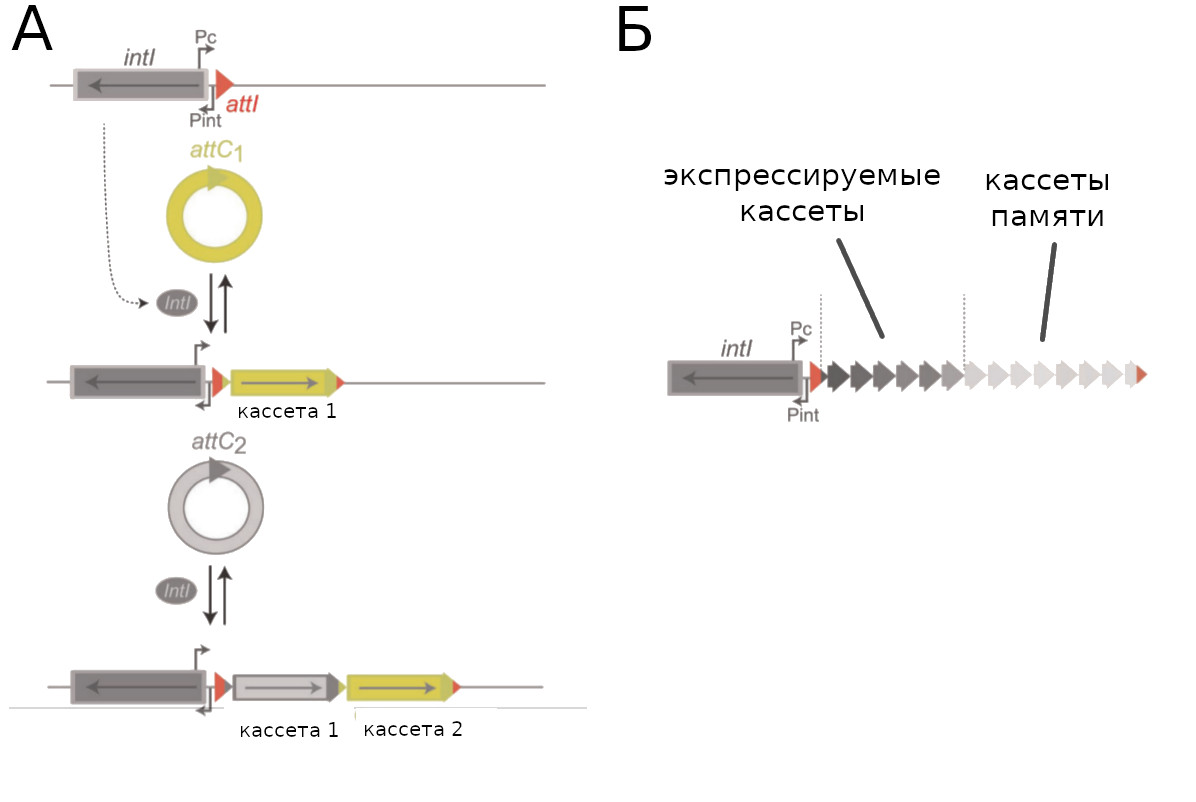
\includegraphics [width=0.85\textwidth] {Dissertation/images/lit/integron.jpg}
  \caption{Устройство и принцип работы оперонов. A) Вставка и вырезание кассет. Интегрон содержит функциональную платформу, состоящую из гена интегразы (intI1), промотора интегразы (Pint), промотора кассеты (Pc) и сайта рекомбинации attI. Б) Уровень экспресии кассет (показан градациями серого цвета) падает по мере удаленности от промотора, только первые из кассет экспрессируются, остальные можно отнести к кассетам ``памяти''. Изображение адаптировано из \cite{boyd2009genomic}.} 
  \label{img:integron}  
\end{figure}

Интегроны содержат ген интегразы (intI), сайт рекомбинации (attI) и промоторные области, необходимые для экспрессии гена интегразы и транскрипции перенесенных в интегрон генов (рисунок~\ref{img:integron}). Эта структура служит платформой для сайт-специфической интеграции нового генетического материала --- генных кассет. Кассеты - кольцевые фрагменты ДНК, как правило состоящие из одного или нескольких генов, лишенных промоторной области. Кассеты также содержат сайт рекомбинации (attC) \cite{gillings2014integrons}. После встраивания, генная кассета становится функциональным геном. Уровень экспрессии встроенных кассет тем выше, чем ближе они расположены к промотору Pc (рисунок~\ref{img:integron}). Интеграза также может случайным образом вырезать генные кассеты и реинтегрировать их на прежнее, либо новое место в интегроне. Таким образом может происходить перестановка генных кассет, с изменение уровня экспрессии встроенных генов. Такая перестановка может служить механизмом подобным простому типу памяти. Кассеты, которые были полезны ранее могут перемещаться в более отдаленные от промотора участки интегрона (например, за счет встраивания новых кассет) что приводит к снижению или прекращению их экспрессии, но не удалению из генома. При последующем возврате к прежним условиям внешней среды, эти кассеты могут подвергнуться процессу перестановки и оказаться вблизи промотора с последующей наработкой с них белков.   

%https://books.google.ru/books?hl=en&lr=&id=oEXzDwAAQBAJ&oi=fnd&pg=PA139&ots=S72ODdX_4B&sig=Qy0nIX9a72y5zxrPvokhgYXw328&redir_esc=y#v=onepage&q&f=false



\subsubsection{Геномные острова}
Понятие геномного острова не определено однозначно. Островами могут называть любые фрагменты ДНК, которые попали в геном в результате горизонтального переноса \cite{langille2010detecting, bazin2020panrgp}. В других работах, под ними понимают такие горизонтально переносимые фрагменты генома, которые содержат в себе "рекомбинационный модуль", включающий в себя интегразу и иные вспомогательные факторы (рисунок~\ref{img:gi}) \cite{boyd2009genomic}. Филогенетический анализ показал, что интегразы, встречающиеся в геномных островах, значительно отличаются от интеграз иных известных мобильных элементов (фагов, интегронов, IS-элементов, интегративных конъюгативных элементов), что может говорить о том, что подобные геномные острова - отдельный вид мобильных элементов генома \cite{boyd2009genomic}. Для ряда геномных островов наблюдалось их вырезание из хромосомы и существование в виде отдельной кольцевой ДНК \cite{blum1994excision, rajanna2003vibrio}. После вырезания, острова могут быть реинтегрированы в хромосому, деградировать либо попасть в новую клетку при помощи общей трансдукции, траснформации либо за счет встраивания в другие мобильные элементы \cite{carpenter2016pathogenicity, pant2020molecular, boyd2009genomic}. На частоту вырезания влияет активность экспрессии рекомбиназ и -- для ряда организмов -- вспомогательных факторов рекомбинации \cite{pant2020molecular}.

\begin{figure}[!ht] 
  \center
  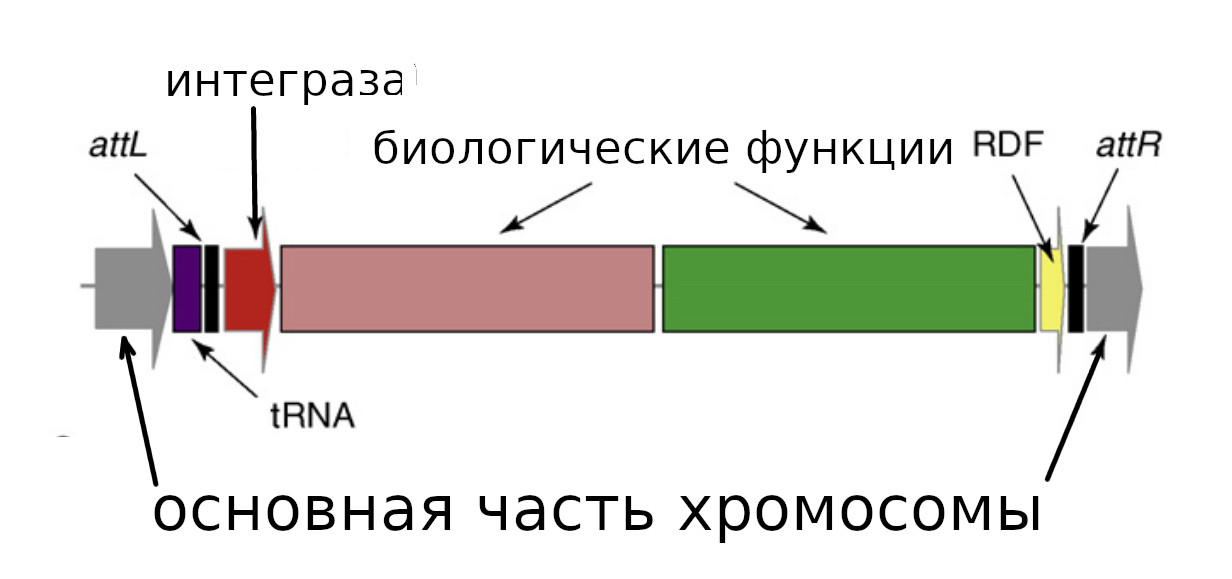
\includegraphics [width=0.7\textwidth] {Dissertation/images/lit/gi.jpg}
  \caption{Схематическое изображение основных компонентов геномного острова. Серые стрелки - основные (коровые) хромосомные гены, фиолетовый прямоугольник представляет - ген тРНК, черные прямоугольники - сайты прикрепления (attL и attR), красная стрелка - ген интегразы, желтая стрелка - фактор направленности рекомбинации (RDF, recombination directionality factor, обнаружены у ряда островов), другие цветные прямоугольники представляют - гены с различными биологическими функциями. Изображение адаптировано из \cite{boyd2009genomic}.} 
  \label{img:gi}  
\end{figure}

Большинство геномных островов, исследованных в работе \cite{boyd2009genomic}, были встроены в гены тРНК, что по мнению авторов обусловлено сайт-специфичностью интеграз и нахождением соответствующих сайтов в генах тРНК. Некоторые геномные острова из рода \textit{Vibrio}, были интегрированы в гены транспортно-матричной РНК (тмРНК). 

Геномные острова отличаются от интегративных конъюгативных элементов тем, что не несут в себе последовательности генов, необходимых для конъюгации, и могут не содержать в своем составе интеграз. Предполагается, что некоторые геномные острова могут передаваться горизонтально за счет использования белков, закодированных в других мобильных элементах (плазмидах, фагах, интегративных конъюгативных элементов) \cite{boyd2009genomic}.

\subsubsection{IS-элементы и транспозоны}
Последовательности вставки или IS-элементы (insertion sequences, IS) являются одними из самых простых мобильных генетических элементов \cite{vandecraen2017impact}. Они представляют из себя короткие (около 1-3 т.п.н.) сегменты ДНК, кодирующие один-два гена и фланкированные инвертированными повторами (рисунок~\ref{img:transposone}А). IS элементы способны к вставке во множество разных мест в. IS-элементы содержат гены транспозазы - белка катализирующего разрезание ДНК и обмен цепями; в некоторых элементах присутствуют регуляторные белки, влияющие на активность транспозазы \cite{siguier2015everyman}. IS-элементы могут перемещаться как внутри генома, так и передаваться между организмами, находясь в составе фагов, плазмид, интегративных конъюгативных элементов \cite{vandecraen2017impact}. Описаны частично деградированные IS-элементы, которые способны к перемещению по геному за счет активности других, интактных, IS-элементов. Такие элементы называются MITE-элементами (miniature inverted repeat transposable elements, MITE) \cite{oggioni1999repeated, siguier2015everyman}. 

IS-элементы играют существенную роль в вариабельности генома \cite{siguier2014bacterial}. Они могут накапливаться в значительном количестве в геноме, а события рекомбинации  между ними часто приводят к удалению геномных фрагментов, что, по-видимому, играет важную роль в уменьшении размера генома видов, перешедших к паразитическому образу жизни \cite{siguier2015everyman}. Встраивание данных элементов в гены, может приводить к потере их функциональности, что в ряде случаев может увеличивать приспособленность организма, например в следствии изменения антигенных детерминант у патогенных микроорганизмов \cite{parkhill2003comparative}. IS-элементы могут увеличивать экспрессию генов за счет образования гибридных промоторов, частично состоящих из фрагментов последовательности IS-элемента \cite{glansdorff1981activation}.

\begin{figure}[!ht] 
  \center
  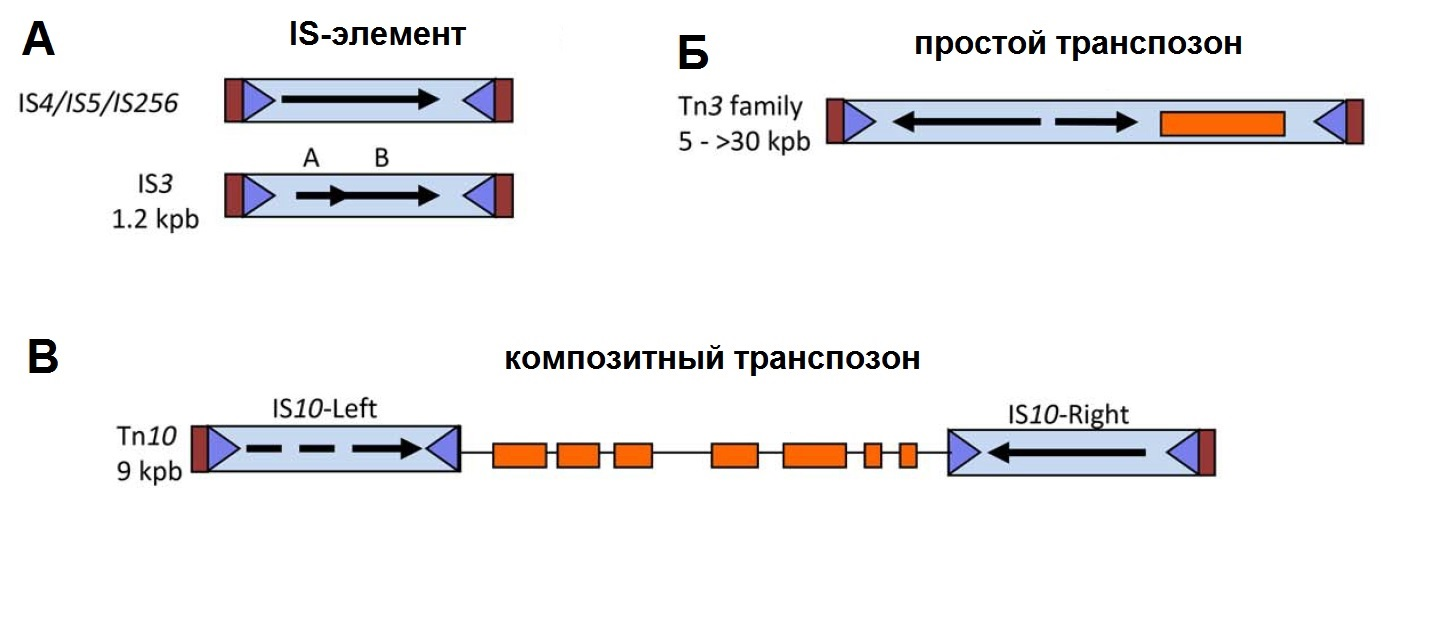
\includegraphics [width=\textwidth] {Dissertation/images/lit/trans.jpg}
  \caption{Схематическое изображение основных типов мобильных элементов, содержащих в себе IS-элементы. IS-элементы показаны голубыми прямоугольниками, концевые инвертированные повторы показаны синими треугольниками, фланкирующие прямые повторы (возникают при интеграции элемента) показаны красными прямоугольниками. Слева указаны семейства IS-элементов и транспозонов, являющиеся их типичными представителями. А) Типичный IS-элемент содержит ген транспозазы и окружен инвертированными и прямыми повторами. Б) Простой транспозон содержит один или несколько генов между повторами. В) Композитный траспозон --- это один или несколько генов, окруженных IS-элементами. Изображение адаптировано из \cite{siguier2015everyman}.} 
  \label{img:transposone}  
\end{figure}

IS элементы могут участвовать в передаче генов, находящихся между ними; такие элементы генома называются составными (композитными или сложными) транспозонами (рисунок~\ref{img:transposone}В) \cite{alton1979nucleotide}. Если IS-элемент содержит в себе один либо несколько карго-генов, то его называют простым транспозоном (рисунок~\ref{img:transposone}Б).  Специфичность встраивания различных транспозонов и IS-элементов значительно различается \cite{wilde2003transposases}.

\subsection{Факторы, влияющие на горизонтальный перенос генов}
Известно, что горизонтальному переносу подвергаются гены всех функциональных категорий, включая и наиболее базовые функции - например, рибосомальные опероны \cite{gogarten2002prokaryotic}. При этом, переноситься могут гены, которые уже присутствуют в геноме реципиента; в таком случае результатом будет не появление нового гена, но замена одно варианта другим. Данный процесс важен для поддержания стабильности генома. Например, для \textit{E. coli} описан сценарий появления склонных к мутациям штаммов за счет поломки генов системы репарации. Затем может происходить исходного уровня мутабельности, за счет горизонтального переноса генов дикого типа \cite{brown2001phylogenetic}. Гипермутабельность может быть полезна в условиях стресса, поскольку может привести к нахождению лучшего в данных условиях варианта генома, а восстановление исходного уровня мутабельности важно для стабилизации нового варианта \cite{caporale2006implicit}.

Для случая переноса новых генов, высказано предположение, что на вероятность того, что ген будет передаваться горизонтально, влияет количество взаимодействий его продукта с другими белками внутри организма \cite{cohen2011complexity}. Согласно данному предположению, чем более тесно связан ген различными взаимодействиями, тем меньше вероятность того, что он будет успешно функционировать в непохожем организме, из-за отсутствия необходимых ему белков-партнеров \cite{novick2020horizontal}.

У ряда естественно-компетентных организмов описаны короткие последовательности (около 12 нуклеотидов), наличие которых увеличивает вероятность горизонтального переноса содержащих их генов. Такие последовательности получили название ``последовательности захвата'' (``uptake sequences''), поскольку они увеличивают вероятность захвата и переноса ДНК. Подобные последовательности описаны у различных представителей семейств Neisseriaceae и Pasteurellaceae \cite{mell2014natural, spencer2016dna}, вида \textit{Haemophilus influenzae} \cite{smith1995frequency}. Различные виды нейсерий обладают немного различными последовательностями захвата \cite{frye2013dialects}; различия в последовательностях захвата связаны со снижением уровня межвидового переноса ДНК. Чаще всего последовательности захвата представлены в генах "домашнего хозяйства"\ и кор-геноме в целом \cite{davidsen2004biased}, что подчеркивает важную роль трансформации в поддержании стабильности геномов за счет исправления мутаций при гомологичной рекомбинации \cite{treangen2008impact}.

Геномные перестройки, обусловленные наличием повторов в геноме могут играть регуляторную роль \cite{смирнов2008механизмы}. Так, для кишечной палочки описана инверсия фрагмента генома, окруженного IS-элементами, и дающая выгоды при голодании бактерий \cite {zinser2003bacterial}.

\subsubsection{Области повышенной частоты горизонтального переноса генов}
Области генома с повышенной частотой событий горизонтального переноса генов --- "горячие точки"\ --- были описаны у ряда бактерий \cite{oliveira2017chromosomal}. Они могут возникать за счет сайт-специфичной интеграции мобильных элементов и находиться в генах тРНК, либо иных генах.  У сальмонелл описана область внутри гена ryeA, служившая сайтом интеграции для чужеродной ДНК \cite{balbontin2008insertion}. Многочисленные изменения генного состава наблюдаются в составе геномных островов, для которых описано наличие консервативных и вариабельных фрагментов \cite{vokes1999aerobactin} (механизм вариабельности при этом остается не известным \cite{myers2006role}). Хорошо изученными точками повышенной изменчивости являются интегроны \cite{boucher2007integrons}. 

Наиболее масштабное исследование "горячих точек"\ горизонтального переноса, которое нам известно, было опубликовано в 2017 году, группой Эдуардо Роча \cite{oliveira2017chromosomal}. Авторы провели исследование уровня изменчивости в 80 бактериальных видах; по их оценкам перенесенные гены сконцентрированы только в ~ 1\% хромосомных областей (горячих точек). Они наблюдали, что большинство мобильных элементов генома и генов устойчивости к антибиотикам находятся в "горячих точках"\, но, при этом, во многих высоко изменчивых областях генома мобильные элементы отсутствуют. 

Также в работе \cite{oliveira2017chromosomal} описано наблюдение, что в окрестности "горячих точек"\ генома наблюдается повышенная частота событий гомологичной рекомбинации. По мнению авторов, это объясняется значительной ролью данного процесса в изменении генного состава в высоковариабельных областях генома.

\section{Биоинформатические методы исследования изменчивости генома}
\subsection{Методы поиска ортологии}
Ортологичные гены --- это гены, происходящие от общего предка (гомологи), связанные с общим предком лишь событиями специализации, без участия событий горизонтального переноса либо дупликаций \cite{fitch1970distinguishing}. Определение ортологиченых генов является важным шагом для филогенетического анализа, предсказания функции генов, сравнительных исследований геномов \cite{glover2019advances}. Поиск ортологов вычислительными методами - сложная задача. Для наиболее точного решения требуется реконструкция генного состава предковых геномов и рассчет эволюционных сценариев для каждого гена с реконструкцией событий дупликации, потери и горизонтального переноса генов \cite{glover2019advances}. Помимо значительной вычислительной сложности, полное решение подобной задачи, требует наличия большого количества геномов, которые были бы репрезентативными для исследуемой группы организмов \cite{theissen2002orthology}. Зачастую, задача поиска ортологов решается приближенными методами. 

Наиболее вычислительно простыми являются методы, основанные на оценке сходства последовательностей. К ним относятся, в частности, методы, основанные на поиске лучших двунаправленных совпадений (best bidirectional hit). В основе лежит предположение, что последовательности ортологичных генов более похожи друг на друга, чем на любые другие последовательности в соответствующих геномах \cite{wolf2012tight}. Данный подход был реализован в таких программах как Hieranoid \cite{schreiber2013hieranoid}, ранних версиях и  публичной базы данных OMA \cite{roth2008algorithm}. Данный подход может учитывать только взаимно-однозначные отношения генов. Если в любой из двух сравниваемых линий произошли дупликации генов, для правильного описания потребуется отношение “один ко многим”\ или “многие ко многим”\. В таких случаях подход, основанный на поиске лучших двунаправленных совпадений, упускает из виду многие истинные ортологи \cite{gabaldon2008large, dalquen2013bidirectional}. 

Широкое распространение получила классификация генов по КОГам - кластерам ортологичных групп (Clusters of Orthologous Groups, COG). КОГи рассчитываются на основе поиска троек наилучших совпадений генов и объединении троек, имеющих общие ребра \cite{tatusov1997genomic}; данный подход не столь консервативен как поиск лучших двунаправленных совпадений и не склонен "пропускать"\ гены, ошибочно не соотнося их с их ортологами \cite{derelle2020broccoli}. Конструирование базы COG было произведено с задействованием курирования полученных кластеров человеком, что было возможно во времена, когда количество прочитанных геномов исчислялось десятками \cite{tatusov2000cog}, но не реализуемо в настоящее время с учетом огромного количества прочитанных геномов. Существуют подходы, основаны на кластеризации генов на основе рассчитанных попарных расстояний между ними, в частности, при помощи метода кластеризации на графах MCL (Markov Cluster Algorithm) \cite{li2003orthomcl, emms2015orthofinder}. В отличие от методов, основанных на поиске лучших двунаправленных совпадений, подход MCL является более инклюзивным (меньшее количество генов ошибочно не соотносятся с группами ортологии). В тоже время он может объединять не ортологичные гены в одну группу, за счет сходства последовательностей \cite{derelle2020broccoli}. Примером реализации данного подхода является программа OrthoFinder \cite{emms2015orthofinder}. На вход ей подаются аминокислотные последовательности белок-кодирующих генов во всех рассматриваемых геномах, после чего происходит запуск попарного выравнивания BLAST (опционально можно использовать diamond \cite{buchfink2015fast}), после чего идет этап кластеризация последовательностей при помощи алгоритма кластеризации на графах MCL \cite{vandongen2000cluster}, полученные в результате кластеры называются ортогруппами. В новой реализации данной программы возможен также дополнительный шаг поиска ортологов на основе филогенетического подхода \cite{emms2019orthofinder}.


Существуют методы поиска ортологов, в которых филогенетический анализ является начальным этапом анализа \cite{gabaldon2008large}. Проводимое вручную сравнение филогенетического дерева, построенного на основе выравнивания гомологичных последовательностей, с деревом рассматриваемых видов служило "классическим"\ методом определения эволюционных сценариев; с появлением большого количества прочитанных геномов подобный анализ стал слишком трудозатратным. Были разработаны автоматические алгоритмы сопоставления генного дерева c деревом видов для получения минимального набора событий дупликации и потери генов, позволяющие объяснить наблюдаемые данные \cite{goodman1979fitting}. Это позволило проводить поиск ортологов на основе филогенетического подхода в масштабе полных геномов \cite{wapinski2007automatic}. Основным ограничением ранних реализаций филогенетического подхода является предположение о том, что филогенетические деревья генов и видов не содержат ошибок, что часто не соответствует реальной ситуации, особенно для деревьев отдельных генов в которых уровень филогенетической информации низок и часто присутствуют одинаковые или очень схожие последовательности \cite{rasmussen2007accurate}. Для борьбы с данным недостатком был предложен подход, при котором фрагменты деревьев с низким уровнем достоверности сначала превращались в полиномии (то есть "схлопывались"\ так, что множество ветвей выходило из одного узла) и затем происходило согласование деревьев для гена и для организмов на основе минимизации получаемых событий дупликаций и потери генов \cite{berglund2006optimal}. 


\subsection{Методы поиска горизонтально переносенных генов}
Для выделения горизонтально перенесенных фрагментов генома, используют различные типы методов \cite{sevillya2020detecting}. В первом типе, определяют фрагменты генома, значительно выделяющиеся по некоторой характеристике (сигнатуре) на фоне остального генома. В качестве сигнатуры может выступать ГЦ-состав, индекс использования кодонов, k-мерный спектр (встречаемость комбинаций из k нуклеотидов) \cite{garcia2000horizontal}. Такой подход применялся с начала 1990 годов (например, \cite{medigue1991evidence} и является наиболее простым в вычислительном плане. Особенно эффективен данный метод для определения недавних событий переноса между филогенетически далекими организмами - за счет дальности организмов ожидаемы значительные отличия в сигнатурах, и эти отличия еще не успели затереться из-за процесса "одомашнивания"\ перенесенного фрагмента ДНК \cite{marri2008gene}. Соответственно, данный тип методов малоприменим для определения переноса между близкими организмами (например, различными штаммами одного вида), поскольку при этом ГЦ состав и иные геномные характеристики ожидаемо будут иметь очень схожие значения. Ограничения данного подхода проистекают также из наличия в геномах вариаций в сигнатурах, не являющихся следствием горизонтального переноса генов \cite{koski2001codon, gogarten2005horizontal}; в частности, отличными от остального генома характеристиками обладают гены мобильных элементов, вирусов и плазмид, а также гены, находящиеся в области конца репликации у ряда бактерий \cite{daubin2003source}. 

Данный тип методов не способен определить донора и реципиента, участвовавших в горизонтальном переносе, задача этих методов --- поиск геномных островов (фрагментов генома, являющихся результатом горизонтального переноса). Примерами реализации данного подхода являются такие программы как Alien hunter \cite{vernikos2006interpolated}, GI hunter \cite{che2014accurate}, GIPSy \cite{soares2016gipsy}. Alien Hunter основан на методе обнаружения атипичных областей в геноме при помощи подхода интерполированных мотивов переменного порядка (IVOM, Interpolated Variable Order Motifs) при анализе содержания G + C, присутствия динуклеотидов и частоте кодонов. Прогнозы оптимизируются с использованием скрытых марковских моделей (HMM) для определения точки входа в атипичные и нетипичные области генома (то есть для уточнения границ горизонтально перенесенного фрагмента). Alien Hunter может делать прогнозы без предварительной аннотации генома. GI hunter тоже основан на методе IVOM, но дополнительно учитывает расположение генов тРНК, наличие интеграз и транспозаз, информацию о генах с высоким уровнем экспрессии, межгенном расстоянии. Все эти данные поступают на вход дерева решений, построенного на обучающей выборке \cite{che2014accurate}. Программа GIPSy также учитывает расположение генов тРНК и генов ассоциированных с мобильными элементами генома, ее отличает функция классификации горизонтально перенесенных фрагментов генома на различные типы: острова патогенности, острова устойчивости к антибиотикам и острова, обеспечивающие симбиоз (symbiotic islands) \cite{soares2016gipsy}. В недавнем сравнении эффективности методов данного типа, наибольшую точность показал Alien Hunter \cite{da2018comparative}.

Второй поход основан на построении филогенетических деревьев отдельно по генам и сравнении их с филогенетическим деревом рассматриваемых организмов (построенном, как правило, на основании общей части геномов (коргенома) либо последовательности 16S рРНК). Гены, для которых эволюционная история плохо совпадает с историей организмов, считаются унаследованными не вертикально (то есть с участием горизонтального переноса либо дубликации) \cite{tofigh2010simultaneous}. Такой подход также начал применяться еще в 1990 годах (например, \cite{smith1992evolution}). Данный подход часто применяется в настоящее время. Например, методом определения горизонтального переноса в базе данных горизонтально-перенесенных генов HGTree \cite{jeong2016hgtree} является метод Ranger-DTL, основанный на филогенетическом подходе \cite{bansal2012efficient}. Ranger-DTL --- это программный пакет для определения эволюции генного семейства с учетом процесса  специализации, дупликации генов, горизонтальному переносу генов и потере генов. Данная программа принимает в качестве входных данных дерево генов и дерево видов и согласовывает их за счет введения предполагаемых событий видообразования, дублирования, передачи и потери генов. Сложность применения данного подхода проистекает от его зависимости от задач, которые сложны и сами по себе - филогенетическая реконструкция и лежащие в ее основе поиск ортологов и множественное выравнивание генов \cite{sevillya2020detecting}. Также, проблему представляет слабость филогенетического сигнала, содержащегося в последовательностях отдельных генов при рассмотрении близкородственных организмов (например, штаммов одного вида). В таком случае деревья, построенные по отдельным генам, содержат много случайных разветвлений с низким уровнем поддержки (например, низкими значениями bootstrap). Для борьбы с возникающими неоднозначностями при реконструкции филогенетического дерева для отдельных генов, в методе GeneRax \cite{morel2020generax} предложено проводить филогенетическую реконструкцию по генам на основе филогенетического дерева для рассматриваемых организмов, за счет этого разрешая возникающие неоднозначности. В качестве входных данных, GeneRax принимает множественное выравнивание для гена и укорененное дерево рассматриваемых организмов (например, построенное на основе общей части геномов). Затем он проводит реконструкцию филогенетического дерева для рассматриваемого гена методом максимального правдоподобия, с учетом различных эволюционных сценариев - событий переноса, дубликации либо потери гена. 

Существуют также программы, реализующие "неявный"\ филогенетический подход. Например, HGTector основан на сравнении сходств белков рассматриваемого генома по отношению к филогенетически близким и филогенетически более далеким организмам. Ряд методов основаны на поиске отличий в генном составе близкородственных геномов: участки которые есть в определенном геноме и при этом отсутствует в геномах большинства филогенетически близких организмов считаются результатами горизонтального переноса генов. Появляются также гибридные методы, использующие в качестве критериев как различие в сигнатурах, так и филогенетическую информацию \cite{sanchez2020shadowcaster}.

Ожидаемо, разнообразие подходов и методов определения горизонтального переноса приводят к разнообразию в получаемых результатах \cite{ragan2006different}.

\subsection{Методы визуализации отличий в геномах}
В данном разделе мы кратко опишем основные методы визуализации, используемые при сравнении геномов.


Одним из первых способов сравнения последовательностей геномов был метод точечных диаграмм сходства, при котором два сравниваемых генома располагаются по двум осям графика, а точками либо линиями отображаются области сходства между геномами (в англоязычной литературе они получили название dot plot alignment). Пример показан на рисунке~\ref{img:comparison}А. Такой способ применим только для пар геномов и сравнительно редко используется в настоящее время.  

Для сравнения нескольких небольших геномов (например, вирусов) или фрагментов больших геномов применяются графики, в которых отдельными горизонтальными линиями показаны геномы, стрелками обозначены гены, а вертикальные линии соединяют гомологичные гены либо области синтении --- схожих по последовательности участков геномов (рисунок~\ref{img:comparison}Г). Несомненным преимуществом такого способа визуализации является наглядность и удобство прослеживания изменения в расположении отдельных генов; метод применим для небольшого числа сравниваемых геномов (порядка 10-20) и небольшом числе генов. 

Схожим образом, можно показывать множественное выравнивание полных последовательностей геномов бактерий, такие графики часто строят в программе Mauve \cite{darling2004mauve} (рисунок~\ref{img:comparison}Б). Сначала происходит поиск блоков синтении. Блоки синтении отображаются прямоугольниками (как правило, цветными) и соответствующие блоки соединяются линиями. Данный подход также ограничен в применимости сравнительно небольшим количеством геномов (порядка 10), после чего полученные визуализации становятся трудны для восприятия. 

Еще одним подходом к визуализации отличий геномов является представление их на круговой диаграмме (рисунок~\ref{img:comparison}В). При этом, один геном выбирается в качестве референса и отображается на внутреннем круге, остальные геномы располагаются на внешних кругах. Для построения данного типа графиков часто применяется программа BRIG (Blast Ring Image Generator) \cite{alikhan2011blast}; она автоматически производит поиск блоков сходства при помощи алгоритма BLAST и позволяет добавить на график различную метаинформацию (ГЦ-состав, добавленные пользователем аннотированные области). Такой подход позволяет наглядно отобразить области, уникальные для референсного генома (например, геномные острова), но не позволяет показать альтернативные варианты генного состава. Количество сравниваемых геномов может быть достаточно большим (многие десятки) без потери информативности визуализации. 


\begin{figure}[!ht] 
  \center
  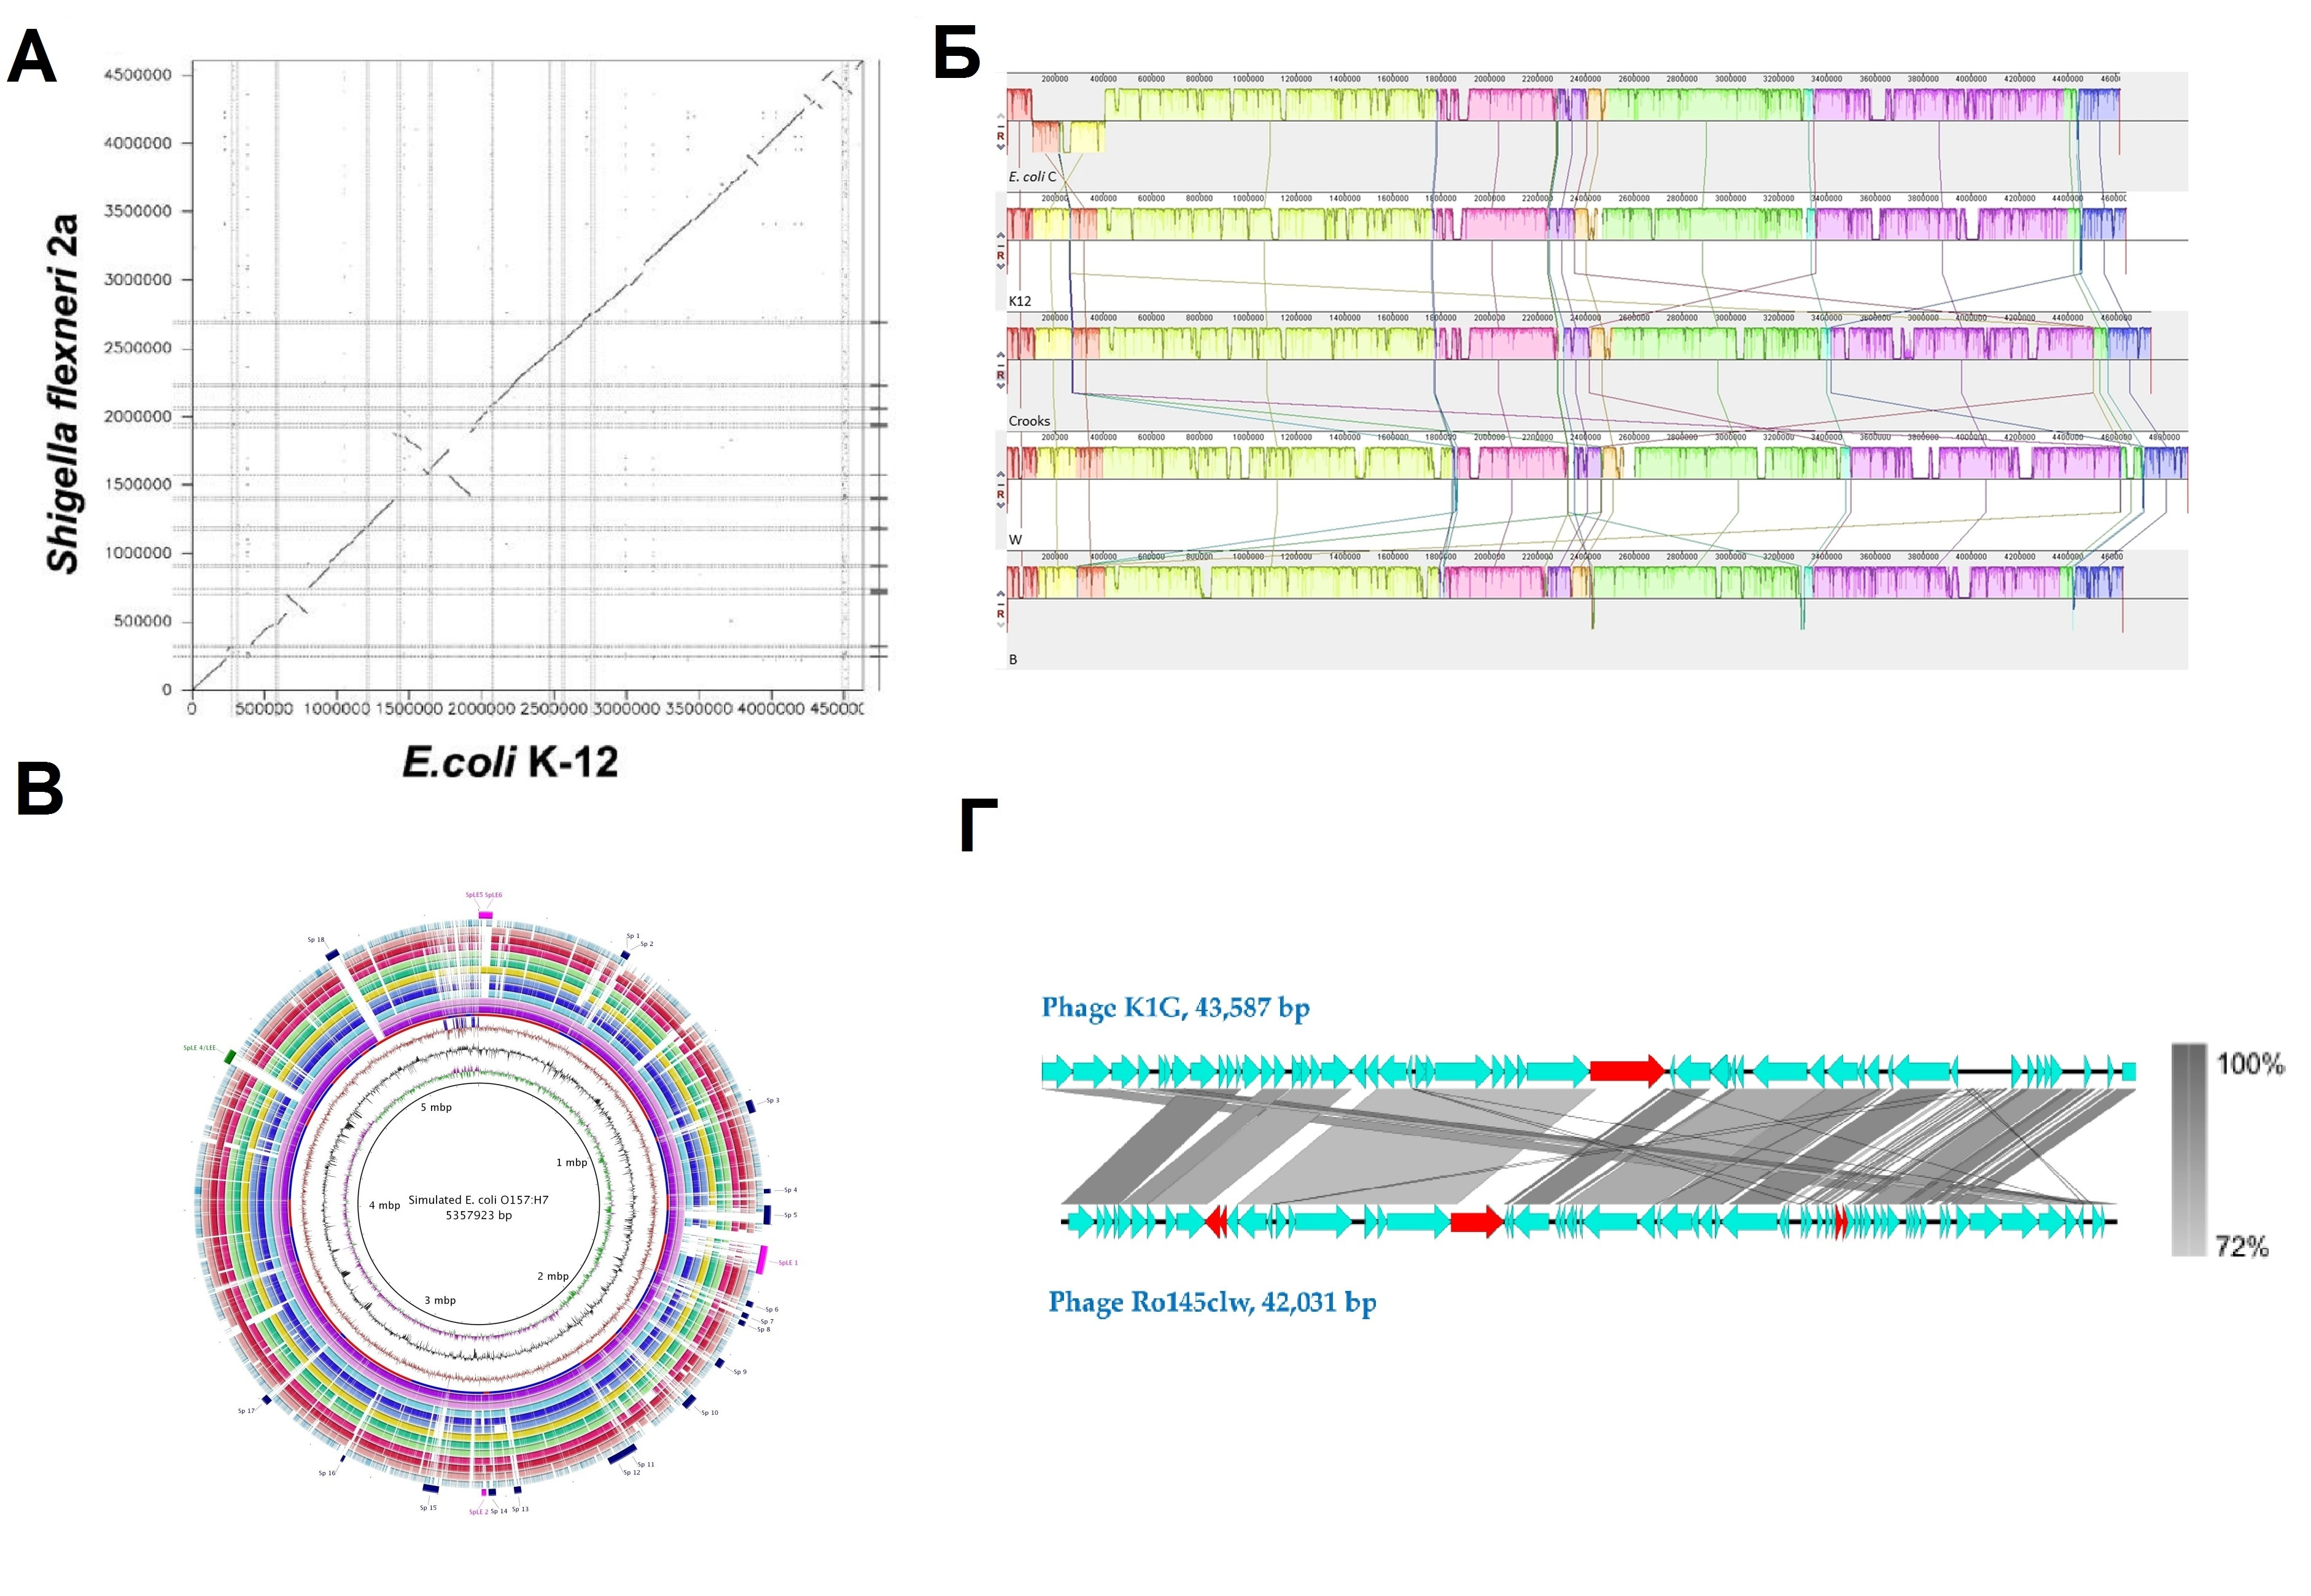
\includegraphics [width=\textwidth] {Dissertation/images/lit/comparisons.jpg}
  \caption{Различые способы визуализации сравнений геномов. А) Сравнение различных штаммов \textit{E. coli}. Координаты геномов сравниваемых штаммов отложены по осям абсцисс и ординат, на пересечении координат ставится точка или проводится линия, при условии совпадения последовательностей по этим координатам. Горизонтальными и вертикальными линиями показано расположение бактериофагов. Изображение адаптировано из \cite{brussow2004phages}, Б) Сравнение различных штаммов \textit{E. coli} при помощи программы Mauve \cite{darling2004mauve}. Показаны крупные блоки синтении; соответствующие блоки соединены линиями. Источник изображения: \cite{krol2019genome}. В) Сравнение геномов различных штаммов \textit{E. coli} при помощи программы BRIG \cite{alikhan2011blast}. Геномы предоставлены в виде колец, внутреннее кольцо соответствует референосному геному. Источник изображения: \cite{alikhan2011blast}. Г) Сравнение состава генов и их расположения в двух фагах. Стрелками обозначены гены, полосами серого цвета показаны схожие последовательности (степень сходства закодирована градиентом серого цвета). Источник изображения: \cite{liao2019characterization}.} 
  \label{img:comparison}  
\end{figure}


\section{Применение графов для анализа геномных данных}

Представление расположения генов в различных геномах в виде графа было применено в работах группы Евгения Кунина в начале 2000х годов \cite{rogozin2002connected, makarova2002dna}. Узлами графа были кластеры ортологичных генов (COG, Clusters of Orthologous Groups of proteins), а ребрами соединялись консервативные пары генов: закодированные на одной цепи, разделенные не более чем двумя генами и представленные в трех и более геномах (из 31 генома, прочтенных к тому моменту).  Целью анализа было нахождение эволюционно устойчивых комбинаций генов. Всего было обнаружено 1505 консервативных пар генов. Большинство пар были представлены лишь в небольшом количестве геномов и только 21 пара генов присутствовала во всех сравниваемых геномах и включала гены рибосомных белков и субъединиц РНК-полимеразы. Также, авторы искали устойчивые кластеры генов, представляющие из себя комбинации устойчивых пар. На рисунке~\ref{img:rogozin_graph} показан граф, представляющий один из обнаруженных кластеров \cite{rogozin2002connected}. Информация об устойчивых кластерах была использована для предсказания функций ранее не охарактеризованных генов архей \cite{makarova2002dna}. В целом, анализ показал, что во многих случаях гены, входящие в кластер, не имели очевидных функциональных связей. По предположению авторов, возможны две альтернативные интерпретации этого результата: 1) гены по соседству только кажутся функционально несвязанными, тогда как в действительности они имеют дополнительные, еще не обнаруженные функции; 2) хотя функциональной связи не существует, продукты этих генов требуются примерно в равных количествах и при тех же условиях, что объясняет преимущество совместного регулирования, обеспечиваемого близким расположением данных генов \cite{rogozin2002connected}. 

\begin{figure}[!ht] 
  \center
  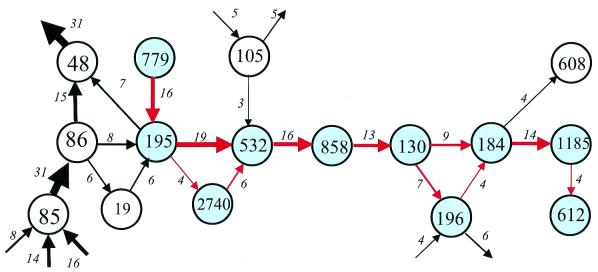
\includegraphics [width=0.8\textwidth] {Dissertation/images/lit/rogozin_graph.jpg}
  \caption{Набор генов, представленный в виде ориентированного графа. Узлы соответствуют кластерам ортологичных генов (COG), номера COG указаны внутри кружков. Иллюстрация взята из работы \cite{rogozin2002connected}. } 
  \label{img:rogozin_graph}  
\end{figure}

% почти граф https://www.ncbi.nlm.nih.gov/pmc/articles/PMC1196056/
В утилите PPanGGOLiN графы, построенные на основе расположения генов (подход, применяемый и в нашей работе), были использованы для классификации генов из пангенома на три категории: устойчивых генов (есть у всех), генов из оболочки (есть у многих) и генов из облака (встречаются у небольшого числа представителей) \cite{gautreau2020ppanggolin}. 
Авторы наблюдали, что доля неконсервативных генов не коррелирует с размером генома.  

Для визуализации графа, который строится в программе PPanGGOLiN, можно использовать графовые редакторы, такие как Gephi (рис~\ref{img:ppangolin}). В декабре 2020 года вышла статья, описывающая модуль программы PPanGGOLiN, предназначенный для поиска геномных островов \cite{bazin2020panrgp}.  

\begin{figure}[!ht] 
  \center
  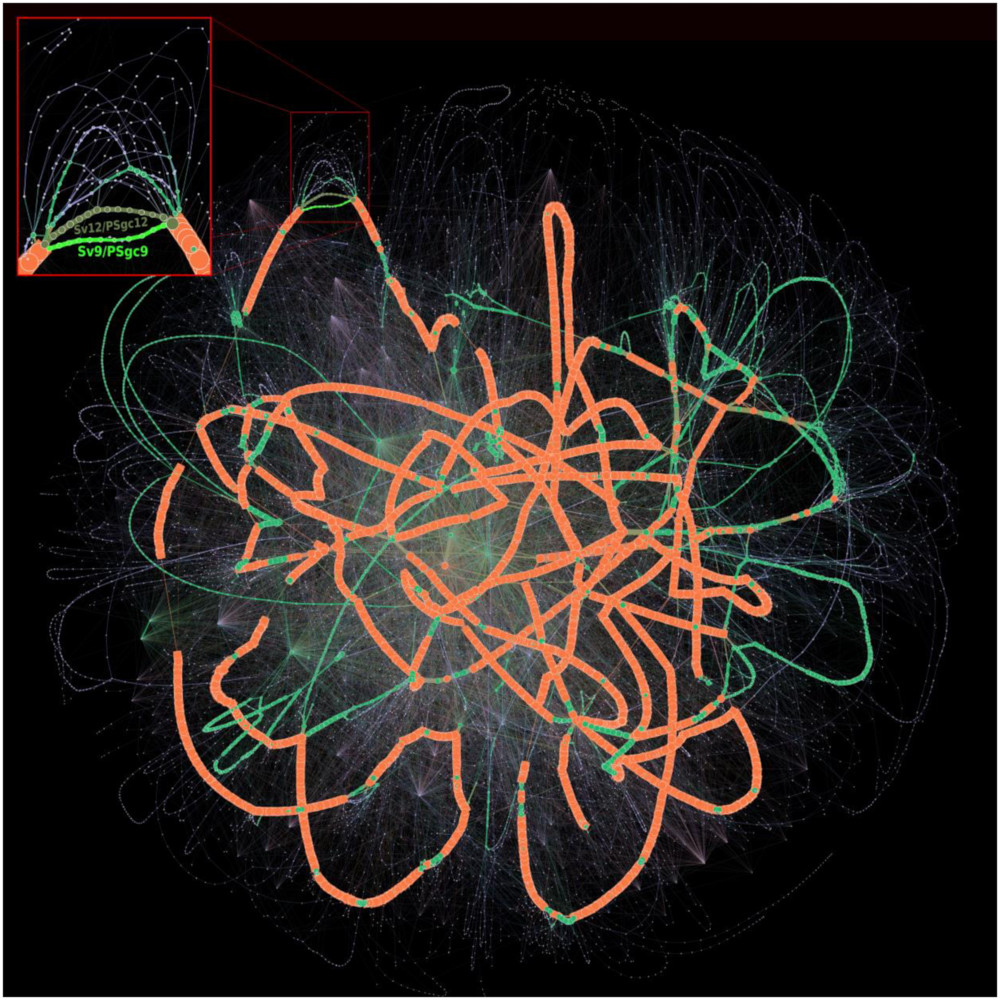
\includegraphics [width=0.6\textwidth] {Dissertation/images/lit/ppangolin.jpg}
  \caption{Пангеномный граф, построенный программой PPanGGOLiN на основе 3117 геномов вида \textit{Acinetobacter baumannii}. Узлы соответствуют семействам генов, ребра соответствуют солокализации генов в геномах. Ребра между генами из устойчивой части генома, оболочки и облака окрашены в оранжевый, зеленый и синий цвета, соответственно. Изображение из публикации \cite{gautreau2020ppanggolin}} 
  \label{img:ppangolin}  
\end{figure}

Также, построение данного типа графов реализовано в пакете FindMyFriends (https://github.com/thomasp85/FindMyFriends) для языка R, предназначенном для проведения пангеномного анализа (поиска групп гомологий, анализа их представленности в геномах). На рис~\ref{img:rfriends} приведен пример визуализации сорасположения генов из различных групп гомологий, выполненный при помощи пакета FindMyFriends.

\begin{figure}[!ht] 
  \center
  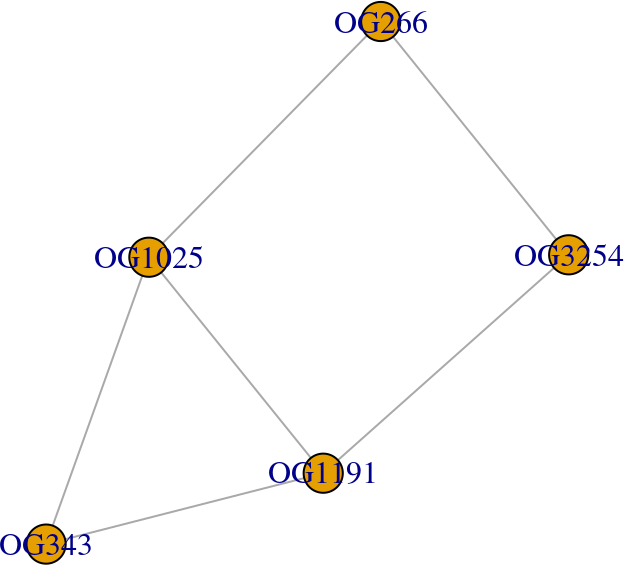
\includegraphics [width=0.5\textwidth] {Dissertation/images/lit/Rfriends.png}
  \caption{Граф сорасположения генов из различных групп гомологий, выполненный при помощи пакета FindMyFriends. Пример из руководства к данному пакету. } 
  \label{img:rfriends}  
\end{figure}


% LDT графы https://arxiv.org/abs/2012.08897

Графы геномной вариабельности, построенные на основе множественного выравнивания, могут быть использованы в качестве референса при картировании прочтений, что улучшает результат картирования (снижает эффект более низкой глубины покрытия в вариабельных участках генома) \cite{paten2011cactus, garrison2018variation}. 

% большой обзор по хромосомной нестабильности https://www.ncbi.nlm.nih.gov/pmc/articles/PMC3957733/

%https://bmcgenomics.biomedcentral.com/articles/10.1186/1471-2164-14-309 -- тут как размывается архитектура в зависимости от филоген. расстояния

\section{Ассоциативная связь болезни Крона с колонизацией \textit{E. coli}}

Болезнь Крона (БК) --- это рецидивирующее воспалительное заболевание кишечника неизвестной этиологии, характеризующееся наличием трансмурального гранулематозного воспаления, диарей, болью в животе, потерей веса, иногда - осложнениями, проявляющихся в иных органах (суставы, печень, глаза) \cite{chervy2020adherent}. Была обнаружена ассоциативная связь между повышенной представленностью \textit{E. coli} в кишечном микробиоме с наличием и тяжестью болезни Крона (как, впрочем, и другими воспалительными заболеваниями кишечника); у пациентов доля кишечной палочки в микробиоте повышена в 10-100 раз (по разным оценкам) по сравнению с ее содержанием у здоровых людей \cite{swidsinski2002mucosal, neut2002changes, miquel2010complete, gevers2014treatment}. Обнаружены мутации в геноме человека, которые увеличивают предрасположенность к болезни Крона. Ряд этих мутаций находится в генах, продукты которых задействованы во взаимодействии человеческого организма и микробиоты  \cite{younis2020inflammatory}. Наиболее вероятным кажется предположение, что в развитии данного заболевания играют роль как факторы внешней среды (включая, нарушение состава микробиоты), так и предрасположенность организма \cite{younis2020inflammatory}. 

Филогенетическое положение изолятов \textit{E. coli} из пациентов с БК значительно варьирует и затрагивает все мажорные филогруппы (A, B1, B2, D) данного организма \cite{rakitina2017genome}. Экспериментально было обнаружено, что ряд изолятов кишечных палочек, полученных от пациентов с БК, оказались способными проникать в эпителиальные клетки кишечника и выживать в макрофагах, что было названо адгезивно-инвазивным фенотипом \cite{boudeau1999invasive, martinez2009molecular,  miquel2010complete}. Согласно мета-анализу, проведенному в 2020 году, кишечная палочка с адгезивно-инвазивным фенотипом встречается у 29\% пациентов с болезнью Крона, что значимо чаще, чем у здоровых людей (у них она встречается в 9\% случаев) \cite{nadalian2020prevalence}. Установить с определенностью генетические детерминанты, позволяющие бактериям приобретать адгезивно-инвазивный фенотип, не удается \cite{shaler2019unique, camprubi2018comparative}. Среди генов, чаще встречающихся у изолятов кишечной палочки из пациентов, по сравнению с изолятами из здоровых людей, в нашем и других исследованиях, были определены гены оперона утилизации 1,2-пропандиола \cite{rakitina2017genome, viladomiu2021adherent, dogan2014inflammation}. Данное вещество является продуктом переработки фукозы комменсальными микробами. У сальмонелл (филогенетически близких к кишечным палочкам патогенных микроорганизмов), утилизация 1,2-пропандиола происходит наиболее эффективно в условиях протекания в кишечнике воспалительной реакции, поскольку при воспалении в просвет выделяются вещества, которые сальмонелла использует как акцепторы электронов. При этом, она становится бенефициаром патологического процесса, а значительная часть иной микрофлоры погибает \cite{faber2017respiration}. Схожий сценарий можно предположить и для кишечной палочки. Вероятно, для нее выгодно провоцировать воспалительную реакции, поскольку это позволяет эффективно утилизировать доступный источник питания и получать доминирующее положение в микробиоме \cite{rakitina2017genome}. Оперон утилизации пропандиола представлен у филогенетически далеких организмов и часто рассматривается как продукт горизонтального переноса генов \cite{anast2020cobalamin, bobik1997propanediol}.

К другим генам кишечных палочек ассоциированными с наличием у их носителя болезни Крона, в разных работах относят гены, вовлеченные в захват железа \cite{rakitina2017genome, nash2010genome}, синтез капсулы \cite{rakitina2017genome, conte2014adherent}, синтез пилей первого типа \cite{cespedes2017genetic}, ген кодирующий белок внешней мембраны OmpC \cite{rolhion2007ompc} и ряд других.


